\documentclass[12pt]{article}
\usepackage{xr-hyper}
\usepackage[unicode]{hyperref}

% \usepackage[hyphens]{url}
\usepackage[dvipsnames,svgnames,x11names]{xcolor}
\usepackage{amsmath,amssymb}
\usepackage{iftex}
\ifPDFTeX
  \usepackage[T1]{fontenc}
  \usepackage[utf8]{inputenc}
  \usepackage{textcomp} % provide euro and other symbols
\else % if luatex or xetex
  \usepackage{unicode-math}
  \defaultfontfeatures{Scale=MatchLowercase}
  \defaultfontfeatures[\rmfamily]{Ligatures=TeX,Scale=1}
\fi
\usepackage{lmodern}
\ifPDFTeX\else  
    % xetex/luatex font selection
\fi
% Use upquote if available, for straight quotes in verbatim environments
\IfFileExists{upquote.sty}{\usepackage{upquote}}{}
\IfFileExists{microtype.sty}{% use microtype if available
  \usepackage[]{microtype}
  \UseMicrotypeSet[protrusion]{basicmath} % disable protrusion for tt fonts
}{}
\makeatletter
\@ifundefined{KOMAClassName}{% if non-KOMA class
  \IfFileExists{parskip.sty}{%
    \usepackage{parskip}
  }{% else
    \setlength{\parindent}{0pt}
    \setlength{\parskip}{6pt plus 2pt minus 1pt}}
}{% if KOMA class
  \KOMAoptions{parskip=half}}
\makeatother
\usepackage{xcolor}
\setlength{\emergencystretch}{3em} % prevent overfull lines
\setcounter{secnumdepth}{5}
% Make \paragraph and \subparagraph free-standing
\makeatletter
\ifx\paragraph\undefined\else
  \let\oldparagraph\paragraph
  \renewcommand{\paragraph}{
    \@ifstar
      \xxxParagraphStar
      \xxxParagraphNoStar
  }
  \newcommand{\xxxParagraphStar}[1]{\oldparagraph*{#1}\mbox{}}
  \newcommand{\xxxParagraphNoStar}[1]{\oldparagraph{#1}\mbox{}}
\fi
\ifx\subparagraph\undefined\else
  \let\oldsubparagraph\subparagraph
  \renewcommand{\subparagraph}{
    \@ifstar
      \xxxSubParagraphStar
      \xxxSubParagraphNoStar
  }
  \newcommand{\xxxSubParagraphStar}[1]{\oldsubparagraph*{#1}\mbox{}}
  \newcommand{\xxxSubParagraphNoStar}[1]{\oldsubparagraph{#1}\mbox{}}
\fi
\makeatother


\providecommand{\tightlist}{%
  \setlength{\itemsep}{0pt}\setlength{\parskip}{0pt}}\usepackage{longtable,booktabs,array}
\usepackage{calc} % for calculating minipage widths
% Correct order of tables after \paragraph or \subparagraph
\usepackage{etoolbox}
\makeatletter
\patchcmd\longtable{\par}{\if@noskipsec\mbox{}\fi\par}{}{}
\makeatother
% Allow footnotes in longtable head/foot
\IfFileExists{footnotehyper.sty}{\usepackage{footnotehyper}}{\usepackage{footnote}}
\makesavenoteenv{longtable}
\usepackage{graphicx}
\makeatletter
\def\maxwidth{\ifdim\Gin@nat@width>\linewidth\linewidth\else\Gin@nat@width\fi}
\def\maxheight{\ifdim\Gin@nat@height>\textheight\textheight\else\Gin@nat@height\fi}
\makeatother
% Scale images if necessary, so that they will not overflow the page
% margins by default, and it is still possible to overwrite the defaults
% using explicit options in \includegraphics[width, height, ...]{}
\setkeys{Gin}{width=\maxwidth,height=\maxheight,keepaspectratio}
% Set default figure placement to htbp
\makeatletter
\def\fps@figure{htbp}
\makeatother

\addtolength{\oddsidemargin}{-.5in}%
\addtolength{\evensidemargin}{-.1in}%
\addtolength{\textwidth}{1in}%
\addtolength{\textheight}{1.7in}%
\addtolength{\topmargin}{-1in}
\makeatletter
\@ifpackageloaded{caption}{}{\usepackage{caption}}
\AtBeginDocument{%
\ifdefined\contentsname
  \renewcommand*\contentsname{Table of contents}
\else
  \newcommand\contentsname{Table of contents}
\fi
\ifdefined\listfigurename
  \renewcommand*\listfigurename{List of Figures}
\else
  \newcommand\listfigurename{List of Figures}
\fi
\ifdefined\listtablename
  \renewcommand*\listtablename{List of Tables}
\else
  \newcommand\listtablename{List of Tables}
\fi
\ifdefined\figurename
  \renewcommand*\figurename{Figure}
\else
  \newcommand\figurename{Figure}
\fi
\ifdefined\tablename
  \renewcommand*\tablename{Table}
\else
  \newcommand\tablename{Table}
\fi
}
\@ifpackageloaded{float}{}{\usepackage{float}}
\floatstyle{ruled}
\@ifundefined{c@chapter}{\newfloat{codelisting}{h}{lop}}{\newfloat{codelisting}{h}{lop}[chapter]}
\floatname{codelisting}{Listing}
\newcommand*\listoflistings{\listof{codelisting}{List of Listings}}
\makeatother
\makeatletter
\makeatother
\makeatletter
\@ifpackageloaded{caption}{}{\usepackage{caption}}
\@ifpackageloaded{subcaption}{}{\usepackage{subcaption}}
\makeatother


\ifLuaTeX
  \usepackage{selnolig}  % disable illegal ligatures
\fi
\usepackage[]{natbib}
\bibliographystyle{apalike}
\usepackage{bookmark}

\IfFileExists{xurl.sty}{\usepackage{xurl}}{} % add URL line breaks if available
\urlstyle{same} % disable monospaced font for URLs
\hypersetup{
  pdftitle={Title},
  pdfauthor={Author 1; Author 2},
  pdfkeywords={3 to 6 keywords, that do not appear in the title},
  colorlinks=true,
  linkcolor={blue},
  filecolor={Maroon},
  citecolor={Blue},
  urlcolor={Blue},
  pdfcreator={LaTeX via pandoc}}

\newcommand{\anon}{0}

%set the key \texttt{anon} to ``0'' to hide the authors and acknowledgements,
%  producing the required anonymized version. 
%Set the key \texttt{anon} to ``1'' to produce the manuscript with author details and
% acknowledgments. 

% Add additional packages here if required
\usepackage{siunitx}

% document
% \usepackage{geometry}
% \setlength{\parindent}{0pt}
% \setlength{\parskip}{1em}
% \renewcommand{\baselinestretch}{1}
% \usepackage[raggedright]{titlesec}

% grafics
\usepackage{graphicx}
\graphicspath{ {./images/sa/} }
\usepackage[export]{adjustbox}
\usepackage{caption}
\usepackage{subcaption}

\usepackage{rotating}
\renewcommand{\topfraction}{.85}
\renewcommand{\bottomfraction}{.7}
\renewcommand{\textfraction}{.15}
\renewcommand{\floatpagefraction}{.66}
\renewcommand{\dbltopfraction}{.66}
\renewcommand{\dblfloatpagefraction}{.66}
\setcounter{topnumber}{9}
\setcounter{bottomnumber}{9}
\setcounter{totalnumber}{20}
\setcounter{dbltopnumber}{9}

\usepackage{tikz}
\usepackage{tkz-graph}  
\usetikzlibrary{shapes.geometric}
\usetikzlibrary{bayesnet, positioning}
\tikzset{ % Define edge styles
    solid edge/.style={->, thick, color=black},
    dashed edge/.style={->, dashed, color=black},
}

% math and text
\usepackage{bm}
\usepackage{mathtools}
\usepackage{amsthm}
\usepackage{nicematrix}

\usepackage[section]{placeins}
\newcommand*{\vertbar}{\rule[-1ex]{0.5pt}{2.5ex}}
\newcommand*{\horzbar}{\rule[.5ex]{2.5ex}{0.5pt}}
\usepackage{xcolor}
\usepackage{tcolorbox}
\usepackage[inline]{enumitem}
\usepackage{soul}

% tables
\usepackage{booktabs}
\usepackage{multirow}
\usepackage{tabularx} 

% circulant notation
\newcommand{\mycirc}[1] {\underline{\bm{#1}}}
\newcommand{\mybcirc}[1] {\underline{\underline{\bm{#1}}}}

% matrix exponential symbol
\newcommand{\eP}{\hspace*{0.015cm}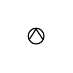
\begin{tikzpicture}[scale=0.1]
      \draw (0,0) circle(1.0);
      \draw (-0.85,-0.4) -- (0,0.9) -- (0.85,-0.4);
    \end{tikzpicture}\hspace*{0.015cm}}

% % algorithms
% \usepackage{algorithm}
% \usepackage{algorithmic}
% \usepackage{float}
% \newfloat{algorithm}{t}{lop}
% algorithms 
\usepackage[ruled,vlined]{algorithm2e}
\SetAlgoNlRelativeSize{0}    % smaller line numbers if needed
\SetAlgoCaptionSeparator{.}  % cleaner caption formatting
\SetAlgoNlRelativeSize{-1}   % even smaller line numbers (optional)


% % External refs
% \externaldocument{supplementary}
% External refs
\makeatletter
\let\XR@bibcite\bibcite
\let\XR@citation\citation
\let\XR@bibdata\bibdata
\let\XR@bibstyle\bibstyle

\renewcommand{\bibcite}[2]{}
\renewcommand{\citation}[1]{}
\renewcommand{\bibdata}[1]{}
\renewcommand{\bibstyle}[1]{}

\externaldocument{supplementary}

\let\bibcite\XR@bibcite
\let\citation\XR@citation
\let\bibdata\XR@bibdata
\let\bibstyle\XR@bibstyle
\makeatother


\begin{document}


\def\spacingset#1{\renewcommand{\baselinestretch}%
{#1}\small\normalsize} \spacingset{1}

%%%%%%%%%%%%%%%%%%%%%%%%%%%%%%%%%%%%%%%%%%%%%%%%%%%%%%%%%%%%%%%%%%%%%%%%%%%%%%


\if0\anon
{
  \title{Bayesian Semi-Blind Deconvolution at Scale}
  \author{
    Guillermina Senn$^{1}$,
    Håkon Tjelmeland$^{1}$,
    Nathan Glatt-Holtz$^{2}$, \\
    Matt Walker$^{3}$,
    and Andrew Holbrook$^{4}$\\[0.5em]
    $^{1}$Department of Mathematical Sciences, NTNU\\
    $^{2}$Indiana University\\
    $^{3}$BP\\
    $^{4}$Department of Biostatistics, UCLA
    }
    \date{}
  \maketitle
  % \thispagestyle{empty}
} \fi

\if1\anon
{
  \bigskip
  \bigskip
  \bigskip
  \begin{center}
    {\LARGE\bf Bayesian Semi-Blind Deconvolution at Scale}
    \end{center}
  \medskip
} \fi

\bigskip

\begin{abstract}
We present a scalable Bayesian semi-blind deconvolution (SBD) framework for regular lattice problems with one-dimensional stationary blur and optional exact image observations. 
The framework is based on a recent approach for seismic SBD that employs data augmentation and cyclic embeddings to allow a scalable Gibbs sampler. 
We make two further methodological contributions. 
First, we derive an explicit eigenvalue-based representation of the posterior computations and Gibbs sampler for the mentioned framework, allowing computations to be performed in the spectral domain. 
Second, we introduce a collapsed Hamiltonian Monte Carlo (HMC) blur update that analytically integrates over the image while retaining scalability under hard image constraints. Simulations and a real seismic problem with about 80{,}000 unknown parameters show that HMC improves exploration in multimodal regimes, while the cheaper Gibbs update is sufficient in the well-constrained real example.
\end{abstract}

\noindent
{\it Keywords:} Inverse problems, image deblurring, cyclic embedding, Fourier transform, collapsed MCMC
\vfill

% \newpage 
\spacingset{1.75} % DON'T change the spacing!


\section{Introduction}
Blind deconvolution (BD) consists of simultaneously recovering an underlying  image and a blur kernel from noisy observations when both are unknown \citep{Campisi2007}. In a discrete setting, the general BD model for a two-dimensional image is mathematically formulated as
\begin{equation} \label{eq:blind_deconvolution_general}
    d(\bm{s}) = (c \star w)(\bm{s}) + e(\bm{s}), \quad  \bm{s} = (s_1, s_2) \in \mathcal{S}_c,
\end{equation}
where $d$ denotes the observations, $c$ the image, $w$ the convolution or blur kernel, $e$ the observational noise, and $\mathcal{S}_c$ is the support of the image.
As described by~\eqref{eq:blind_deconvolution_general}, BD is a non-linear, ill-posed inverse problem because different blur-image combinations can generate the observed data. Reviews of deterministic and statistical techniques to solve the inverse problem can be found in \citet{levin2011understanding} and \citet{chaudhuri2014blind}.

We adopt the Bayesian approach to BD, where image, blur and error are treated as random variables and the image and blur prior distributions regularize the solution. When additional information on the image or blur is available, for instance in the form of positivity or sum-to-one constraints on the blur and affine constraints on the image, the problem is called semi-blind deconvolution (SBD). The posterior distribution provides a full solution to the BD inverse problem together with uncertainty quantification. Except for a few exceptions, this posterior distribution is intractable and must be estimated.

Markov Chain Monte Carlo (MCMC) is the gold standard for generating asymptotically exact samples from any Bayesian posterior. Among widely used MCMC algorithms we count Metropolis-Hastings \citep{metropolis1953equation,Hastings1970}, the Gibbs sampler \citep{GemanGeman1984}, and Hamiltonian Monte Carlo (HMC; \citet{Duane1987}). Typically, these standard algorithms do not scale computationally well with dimension of the parameter space and the data. If one is willing to sample from an approximate posterior, Variational Bayes (VB) can offer a computationally attractive alternative, sometimes allowing more flexibility in the choice of prior distributions for the image and the blur; works like \citet{babacan2012bayesian}, \citet{molina2006}, \citet{likas2004}, and \citet{Tzikas2009} use VB to approximate the posterior of their hierarchical Bayesian models.

The literature on MCMC-based Bayesian approaches for the general model in~\eqref{eq:blind_deconvolution_general} is more limited. \citet{orieux2010bayesian} propose a conjugate model for myopic deconvolution with uniform blur parameters prior and Gaussian image and noise, the latter admitting a Fourier representation that allows an efficient, spectral-based Metropolis-within-Gibbs sampler. \citet{Park2012} consider a similar approach but with image and blur priors that do not allow the same spectral simplifications. 

One application domain where solving BD problems is essential is geophysical research, and seismic analysis of subsurface reservoirs in particular. In seismic imaging, and due to the acquisition method, the processed observed data is often modeled by a convolutional relation that links a reflectivity series to an effective seismic wavelet, plus additive noise. In addition, it is common to have reflectivity observations along one or several wells drilled vertically across the subsurface, which act as additional image information and thus makes some problems in seismic inversion a natural instance of SBD. Statistical estimation of the reflectivity and wavelet is widely used in practice and can improve the interpretation of reservoir structure and subsurface properties. We refer to \citet{SheriffGeldart1995} for a detailed overview of seismic reflection data and to \citet{KaaresenTofinn1993,GranaEtAl2022} for representative Bayesian formulations.

In the seismic SBD literature, \citet{BulandOmre2003a, BulandOmre2003b} proposed a Bayesian conjugate model for a version of~\eqref{eq:blind_deconvolution_general} that assumes a \textit{spatially invariant}, one-dimensional blur kernel.
%acting vertically on each trace. 
Namely, if $s_1$ and $s_2$ denote the vertical and lateral coordinates respectively, the discrete convolutional model becomes
\begin{equation}
    d(s_1,s_2)
    =
    \sum_{\tau \in \mathcal{S}_w}
    c(s_1-\tau,s_2)\,w(\tau)
    +
    e(s_1,s_2),
    \label{eq:blind_deconvolution}
\end{equation}
where $c$ and $e$ are spatial fields defined on the two-dimensional image domain and $w$ is a one-dimensional blur kernel defined on the blur support $\mathcal{S}_w$. Thus, convolution is performed independently along each vertical trace using the same kernel at every lateral location. 

In this important work from \citet{BulandOmre2003a, BulandOmre2003b}, the reflectivity image, well reflectivity, noise and seismic wavelet are treated as multivariate Gaussians with stationary, separable correlation structures. The associated Gibbs sampler scales cubically in the data size, and consequently wavelet estimation is restricted to a small subset of image traces. 

\citet{Senn2025} extend the method to allow wavelet estimation from all image traces. Their strategy employs data augmentation and an extended cyclic model formulation. The cyclic formulation combined with the stationarity and separability assumptions of the Gaussian correlation matrices allows expensive computations in the Gibbs sampler to be performed with the fast Fourier transform (FFT).
The Gaussian full conditionals are then sampled using conditioning by Kriging, which imposes the observed data and the exact image observations, such as well reflectivity values, as hard linear constraints.

Our contribution is threefold. First, we formulate the model outside its original seismic setting.
Second, we derive an explicit eigenvalue-based representation of the posterior computations and Gibbs sampler, so that the main updates can be implemented directly in the spectral domain. 
Third, we introduce a marginal blur update obtained by analytically integrating out the image from the joint blur-image conditional and sampling the resulting marginal blur conditional with Hamiltonian Monte Carlo (HMC). 

The marginal update is motivated by the collapsed MCMC sampling literature, where integrating out nuisance variables is known to reduce correlations in the Markov transition and often improves mixing \citep{Liu2008}. Although analytical formulas for the potential and gradient in HMC for the target distribution are available, the image hard constraints complicate their efficient evaluation and we exploit algebraic structure to retain scalability.

The rest of the article is organized as follows. In Section~\ref{sec:preliminaries} we introduce the efficient Gaussian sampling techniques used throughout the article. In Section~\ref{sec:model} we describe the cyclic Bayesian model. In Section~\ref{sec:mcmc} we present the MCMC algorithm and its scalable implementation. 
In Section~\ref{sec:results} we demonstrante the scalability of the method and compare the conditional Gibbs blur update and the marginal HMC blur update, first on simulated data, where we isolate the role of the exact image observations, and then on a real seismic dataset from a gas reservoir offshore Egypt corresponding to a posterior with $\sim 80$k parameters.
We conclude in Section~\ref{sec:conclusion}.


\section{Preliminaries} \label{sec:preliminaries}
In this section we review Gaussian conditional distributions, conditioning by Kriging (CBK), circulant matrices, and discrete Fourier transform (DFT) techniques used throughout to efficiently sample from Gaussian distributions.

\subsection{Conditional Gaussian distributions}

Let $\bm{x} \in \mathbb{R}^n$ be a random vector that follows a Gaussian distribution with mean $\bm{\mu}$ and covariance matrix $\bm{\Sigma}$. We express this as $\bm{x} \sim N_n(\bm{\mu}, \bm{\Sigma})$ and denote the density of this distribution by $p(\bm{x})$. 
Let $\bm{A}$ be a $k \times n$ constant matrix, let $\bm{e}\sim N_k(\bm{0}, \bm{\Sigma}_e)$, and suppose we observe $\bm{y}=\bm{A}\bm{x}+\bm{e}$.
Then the distribution of $\bm{x}$ conditional on $\bm{y}$ is also Gaussian, $\bm{x}|\{\bm{A}\bm{x}+\bm{e}=\bm{y}\} \sim N_n(\tilde{\bm{\mu}}, \tilde{\bm{\Sigma}})$, with conditional parameters
\begin{equation} \label{eq:gaussian_conditional_pars}
\begin{split}
    \tilde{\bm{\mu}}&= \bm{\mu} + \bm{\Sigma} \bm{A}^{\top} (\bm{A} \bm{\Sigma} \bm{A}^{\top} + \bm{\Sigma}_e)^{-1} (\bm{y} - \bm{A} \bm{\mu}),\\
    \tilde{\bm{\Sigma}} &= \bm{\Sigma} - \bm{\Sigma} \bm{A}^{\top} (\bm{A}\bm{\Sigma} \bm{A}^{\top} + \bm{\Sigma}_e)^{-1}\bm{A}\bm{\Sigma},
\end{split}
\end{equation}
and density denoted by $p(\bm{x} | \{\bm{A}\bm{x}+\bm{e}=\bm{y}\} )$.

% Let $\bm{x} \in \mathbb{R}^n$ be a random vector that follows a Gaussian distribution with mean $\bm{\mu}$ and covariance matrix $\bm{\Sigma}$. We express this as $\bm{x} \sim N_n(\bm{\mu}, \bm{\Sigma})$ and denote the density of this distribution by $p(\bm{x})$. 
% Let $\bm{A}$ be a $k \times n$ constant matrix and let $\bm{e}\sim N_k(\bm{0}, \bm{\Sigma}_e)$. Then the distribution of $\bm{x}$ conditional on the linear combination $\bm{A}\bm{x} + \bm{e}$ is also Gaussian, $\bm{x}|\{\bm{A}\bm{x} + \bm{e}\} \sim N_n(\tilde{\bm{\mu}}, \tilde{\bm{\Sigma}})$ with conditional parameters
% \begin{equation} \label{eq:gaussian_conditional_pars}
% \begin{split}
%     \tilde{\bm{\mu}}&= \bm{\mu} + \bm{\Sigma} \bm{A}^{\top} (\bm{A} \bm{\Sigma} \bm{A}^{\top} + \bm{\Sigma}_e)^{-1} (\bm{Ax} + \bm{e} - \bm{A \mu}),\\
%     \tilde{\bm{\Sigma}} &= \bm{\Sigma} - \bm{\Sigma} \bm{A}^{\top} (\bm{A}\bm{\Sigma} \bm{A}^{\top} + \bm{\Sigma}_e)^{-1}\bm{A}\bm{\Sigma},
% \end{split}
% \end{equation}
% and density denoted by $p(\bm{x} | \{\bm{A}\bm{x} + \bm{e}\} )$. 

The conditional covariance $\tilde{\bm{\Sigma}}$ in~\eqref{eq:gaussian_conditional_pars} is not always full rank. For example, consider the situation when $\bm{e}=\bm{0}$ and $k<n$; then $\tilde{\bm{\Sigma}}$ has rank $n-k$ and the conditional density $p(\bm{x}|\bm{A}\bm{x})$ is singular. 
Assume in addition that $\bm{A}$ is a selection matrix of zeros and ones that picks out $k$ elements of $\bm{x}$ such that the hard linear constraints $\bm{A} \bm{x} = \bm{b}$ assign the values stored in a constant vector $\bm{b}\in \mathbb{R}^k$ to these $k$ elements. We then have that the conditional distribution of $\bm{x}$ given the hard linear constraints is a singular Gaussian, i.e. $\bm{x}^{\star}=\bm{x}|\{\bm{A}\bm{x}=\bm{b}\}\sim N_n(\bm{\mu}^{\star}, \bm{\Sigma}^{\star})$, with parameters $\bm{\mu}^{\star}$ and $\bm{\Sigma}^{\star}$ obtained by setting $\bm{e}=\bm{0}$, $\bm{\Sigma}_e = \bm{0}$, and $\bm{Ax}=\bm{b}$ in~\eqref{eq:gaussian_conditional_pars}, and density denoted by $p(\bm{x}^{\star})$.

A distribution for the non-constrained elements in $\bm{x}^{\star}$ can be derived as follows. Let $\bm{A}^C$ be the $(n-k) \times n$ selection matrix that selects from $\bm{x}$ those $n-k$ elements not selected by $\bm{A}$ such that $\bm{x}_u^{\star} = \bm{A}^C \bm{x}^{\star} $ contains the $n-k$ non-constrained elements in $\bm{x}^{\star}$. Then $\bm{x}_u^{\star}\sim N_{n-k}(\bm{A}^C\bm{\mu}^{\star}, \bm{A}^C \bm{\Sigma}^{\star} (\bm{A}^{C})^{\top})$. Denoting the (non-singular) density of this distribution by $q(\bm{x}_u^{\star})$, we have that $q(\bm{x}_u^{\star}) = p(\bm{x}^{\star})$, as shown in Section~\ref{sec:equal_densities} in the Supplementary Material (SM). 

To sample $\bm{x}^{\star}$ one could compute $\bm{\mu}^{\star}$ and $\bm{\Sigma}^{\star}$ explicitly with~\eqref{eq:gaussian_conditional_pars}, decompose the singular $\bm{\Sigma}^{\star}$, and sample from the resulting Gaussian with the classic approach, a computationally intensive procedure. Algorithm~\ref{alg:cbk} presents \textit{conditioning by Kriging}, an alternative  sampling approach that avoids the decomposition and explicit computation of the conditional parameters, and that can be computationally efficient for $k<n$ \citep{RueHeld2005}. 
A sample $\bm{x}^{\star}_u$ can be obtained by subsetting the non-constrained elements in the sample $\bm{x}^{\star}$.

\begin{algorithm}[t]
\caption{Sample $\bm{x}^{\star} \sim N_{n}(\bm{\mu}^{\star}, \bm{\Sigma}^{\star})$ with conditioning by Kriging.}
\label{alg:cbk}
\SetAlgoNlRelativeSize{-3}
\DontPrintSemicolon
1. Sample $\bm{x} \sim N_n(\bm{\mu}, \bm{\Sigma})$ with traditional algorithms. \\
2. Return $\bm{x}^{\star} = \bm{x} - \bm{\Sigma} \bm{A}^{\top} (\bm{A} \bm{\Sigma} \bm{A}^{\top})^{-1} (\bm{A}\bm{x} - \bm{b})$.
\end{algorithm}

\subsection{Circulant matrices and the DFT}
A \textit{circulant} matrix of order $n$, denoted hereafter with a single underline, is a matrix of the form 
\begin{equation}\label{circMatrix}
\begin{split}
\mycirc{C} &= \mbox{circ}(c_0, c_1, \dots, c_{n-1}) =\begin{pmatrix}
c_{0} & c_{1} & \dots & c_{n-1}\\ 
c_{n-1} & c_{0} & \dots & c_{n-2} \\ 
\vdots & \vdots &  & \vdots \\
c_{1} & c_{2} & \dots & c_{0}
\end{pmatrix},
\end{split}
\end{equation}
with each row a cyclic shift of the previous row. The whole matrix is determined by the first row $\bm{c} = (c_0, c_1, \dots, c_{n-1})$, called the base of the circulant \citep{Davis1979}. 
% We use a single underline to denote that a matrix is circulant. 

A circulant matrix $\mycirc{C}$ of order $n$ is always diagonalizable as
\begin{align} \label{eq:diagonalization_circ}
  \mycirc{C} = \bm{F}_n^H\bm{\Lambda}_{\mycirc{C}}\bm{F}_n,
\end{align}
where $\bm{\Lambda}_{\mycirc{C}}=\mbox{diag}(\bm{\lambda}_{\mycirc{C}})$ is a square diagonal matrix with the eigenvalues
$\bm{\lambda}_{\mycirc{C}}=(\lambda_1,\ldots,\lambda_n)^{\top}$ of $\mycirc{C}$ on the diagonal, $^H$ denotes the Hermitian, and $\bm{F}_n$ is the so called Fourier matrix of order $n$, defined by
\begin{equation} 
    \left [ \bm{F}_n \right ]_{ij} = \frac{1}{\sqrt{n}} \exp{ \left ( \frac{2\pi \mathsf{i}}{n} \right )}^{(i-1)(j-1)}, \quad 1 \le i, j \le n.
\end{equation}

The diagonalization in~\eqref{eq:diagonalization_circ} defines the following simple relation between the base $\bm{c}$ and the vector of eigenvalues $\bm{\lambda}_{\mycirc{C}}$,
\begin{align} \label{eq:eigenvalues_fft_matrix}
  \bm{\lambda}_{\mycirc{C}} = \sqrt{n}\bm{F}_n\bm{c} \hspace*{0.4cm}\Leftrightarrow\hspace*{0.4cm}
  \bm{c}=\frac{1}{\sqrt{n}}\bm{F}_n^H \bm{\lambda}_{\mycirc{C}},
\end{align}
where the equivalence follows because $\bm{F}_n^{-1}=\bm{F}_n^H$. 
With the diagonalization convention used, the multiplication of $\bm{F}_n$ with a vector $\bm{x}$ returns the DFT of $\bm{x}$, and the multiplication of $\bm{F}_n^H$  with $\bm{x}$ returns its inverse DFT (IDFT). As the complexity of both DFT and IDFT computed with the FFT is ${\cal O}(n\log n)$, the computation of $\bm{\lambda}_{\mycirc{C}}$ from $\bm{c}$, and vice versa, can be done efficiently.

The diagonalization in~\eqref{eq:diagonalization_circ} implies that the class of circulants of order $n$ is closed under eigenvalue-based operation, such as linear combinations, matrix multiplication, transposition and inversion \citep{Davis1979}.
For example, let $\mycirc{A} = [a_{ij}]$ and $\mycirc{B}$ be circulants of order $n$ with bases $\bm{\alpha}$ and $\bm{\beta}$ and eigenvalues $\bm{\lambda}_{\mycirc{A}}$ and $\bm{\lambda}_{\mycirc{B}}$ organized in the diagonal matrices $\bm{\Lambda}_{\mycirc{A}} = \mbox{diag}(\bm{\lambda}_{\mycirc{A}})$ and $\bm{\Lambda}_{\mycirc{B}} = \mbox{diag}(\bm{\lambda}_{\mycirc{B}})$, respectively, and consider the multiplication of $\mycirc{A}$ with $\mycirc{B}$. Then $\mycirc{C} = \mycirc{A}\mycirc{B} \iff \bm{\lambda}_{\mycirc{C}} = \bm{\lambda}_{\mycirc{A}} \odot \bm{\lambda}_{\mycirc{B}}$, where $\bm{\lambda}_{\mycirc{C}}$ are the eigenvalues of $\mycirc{C}$ and $\odot$ represents element-wise or Hadamard product, because
$\mycirc{A}\mycirc{B} = \bm{F}_n \bm{\Lambda}_{\mycirc{A}} \bm{F}_n^H \bm{F}_n \bm{\Lambda}_{\mycirc{B}} \bm{F}_n^H = \bm{F}_n \bm{\Lambda}_{\mycirc{A}} \bm{\Lambda}_{\mycirc{B}} \bm{F}_n^H$. 
The practical implication is that eigenvalue-based operations among circulants have computational cost $\mathcal{O}(n)$ once the eigenvalues of the matrices have been obtained in $\mathcal{O}(n \log n)$ with the FFT.


The Kronecker product $\otimes$ between two circulants $\mycirc{A}$ and $\mycirc{B}$ of order $m$ and $n$, respectively, with bases $\bm{\alpha}$ and $\bm{\beta}$ defines a \textit{block-circulant with circulant blocks} (BCCB) matrix of type $(m, n)$, denoted hereafter with a double underline, which is a matrix of order $mn$ with form
\begin{equation} \label{eq:kronecker_product}
\mybcirc{C} = \mycirc{A} \otimes \mycirc{B} = 
\begin{pmatrix}
a_{00} \mycirc{B} & \cdots & a_{0,m-1} \mycirc{B}\\ 
\vdots & \ddots & \vdots \\
a_{m-1,0} \mycirc{B} & \cdots & a_{m-1,m-1} \mycirc{B}
\end{pmatrix}.
\end{equation}
Each block-row in $\mybcirc{C}$ is a cyclic block-shift of the previous block-row, and the whole matrix is specified by its $n \times m$ base $\bm{\Pi}=\bm{\beta} \bm{\alpha}^{\top}$, so that $\operatorname{vec}(\bm{\Pi})=\bm{\alpha}\otimes\bm{\beta}$. 

A BCCB is always diagonalized by the unitary matrix $\bm{F}_m \otimes \bm{F}_n$ as 
\begin{equation} \label{eq:diagonalization_2d}
    \mybcirc{C} = (\bm{F}_m \otimes \bm{F}_n)^H \bm{\Lambda}_{\mybcirc{C}}(\bm{F}_m \otimes \bm{F}_n),
\end{equation}
where $\bm{\Lambda}_{\mybcirc{C}}$ is a diagonal matrix with the $mn$ eigenvalues $\bm{\lambda}_{\mybcirc{C}} = (\bm F_m \otimes \bm F_n)\operatorname{vec}(\bm\Pi)$ of $\mybcirc{C}$ in its diagonal. 
The multiplication of $\bm{F}_m \otimes \bm{F}_n$ with a vector $\bm{x}$ is known as the two-dimensional DFT (DFT2) of $\bm{x}$, and correspondingly $(\bm{F}_m \otimes \bm{F}_n)^H\bm{x}$ gives its two-dimensional IDFT (IDFT2). 
The diagonalization in \eqref{eq:diagonalization_2d}
implies that the class of BCCB matrices of type $(m, n)$ is closed under eigenvalue-based operations.

For notational convenience, we avoid repeatedly writing the Fourier diagonalizations of circulant and BCCB matrices. Throughout, for any circulant or BCCB matrix $\mybcirc{A}$, $\bm{\lambda}_{\mybcirc{A}}$ denotes its eigenvalue vector and
$\bm{\Lambda}_{\mybcirc{A}}=\operatorname{diag}(\bm{\lambda}_{\mybcirc{A}})$
the corresponding diagonal eigenvalue matrix. Thus
$
\bm{\Lambda}_{\mybcirc{A}}\hat{\bm{x}}
=
\bm{\lambda}_{\mybcirc{A}}\odot\hat{\bm{x}},
$
and convolutions on the cyclic lattice are equivalent to componentwise multiplication in the Fourier domain.

\subsection{Stationary Gaussian distributions on cyclic lattices}

Consider a regular $n_v \times n_h$ lattice with $n=n_v n_h$ nodes. We define the periodic vertical and horizontal separations between two nodes $(i,j)$ and $(k,l)$ as
\[
    h_v(i,k)=\min(|i-k|,n_v-|i-k|)
    \qquad \mbox{and} \qquad
    h_h(j,l)=\min(|j-l|,n_h-|j-l|).
\]
With this setup, the lattice acquires periodic boundary conditions in both directions, the one-dimensional distance matrices $\mycirc{H}_h=[h_h(j,l)]$ and $\mycirc{H}_v=[h_v(i,k)]$ in the horizontal and vertical directions are circulant, and separable covariance matrices built from these distances are BCCB.

% Consider a regular $n_v \times n_h$ lattice with $n=n_v n_h$ nodes, with distance between two nodes $(i, j)$ and $(k, l)$ defined as $h((i,j), (k,l)) := h_{ik}\,h_{jl}$, where $h_{ik} = \text{min}(|i-k|, n_v-|i-k|)$ and $h_{jl} = \text{min}(|j-l|, n_h-|j-l|)$. In other words, the distance between any two nodes is given by the product of the great-circle distance in each direction. With this setup, the lattice acquires periodic boundary conditions in both directions, the  one-dimensional distance matrices $\mycirc{H}_h=[h_{jl}]$ and $\mycirc{H}_v=[h_{ik}]$ in the horizontal and vertical directions are circulant, and the spatial lattice distance matrix $\mybcirc{H}=\mycirc{H}_h \otimes \mycirc{H}_v$ is BCCB.  

Let $\bm{x}$ be a random field on this cyclic lattice and let $x_{ij}$ denote the random variable associated with node $(i, j)$. 
Next, assume stationary covariance functions in each direction. Then, the horizontal and vertical covariance matrices $\mycirc{\Sigma}_v$ and $\mycirc{\Sigma}_h$ inherit the circulant structure of the distance matrices, and a separable spatial covariance $\mybcirc{\Sigma}=\mycirc{\Sigma}_h \otimes \mycirc{\Sigma}_v$
is BCCB.
Assuming that $\bm{x}$ has a Gaussian distribution with parameters $\mybcirc{\Sigma}$ and $\bm{\mu}$, then
\begin{equation}
    \bm{x}\sim N_n(\bm{\mu}, \mybcirc{\Sigma}) \iff \hat{\bm{x}} \sim N_n(\hat{\bm{\mu}}, \bm{\Lambda}_{\mybcirc{\Sigma}}),
\end{equation}
where we use the notation $\hat{\bm{x}} = \mbox{DFT2}(\bm{x})$, and Algorithm~\ref{alg:fft_2d_mvn_FD} can be used to sample $\hat{\bm{x}}$ in the Fourier domain in $\mathcal{O}(n)$. Then, $\bm{x} = \text{Re}(\mbox{IDFT2}(\hat{\bm{x}}))$ in the original domain can be found in $\mathcal{O}(n \log n)$. 
When $\mybcirc{\Sigma}$ is circulant instead of BCCB, the (I)DFT2 reduces to the (I)DFT. 

\begin{algorithm}[t]
\caption{Sampling $\hat{\bm{x}} \sim N_{n}(\hat{\bm{\mu}}, \bm{\Lambda}_{\mybcirc{\Sigma}})$ with $\hat{\bm{\mu}} = \mbox{DFT2}(\bm{\mu})$ and $\bm{\Lambda}_{\mybcirc{\Sigma}} = \mbox{diag}(\bm{\lambda}_{\mybcirc{\Sigma}})$.}
\label{alg:fft_2d_mvn_FD}
\SetAlgoNlRelativeSize{-3}
\DontPrintSemicolon
1. Sample $\bm{z}$, a $n \times 1$ vector where $\text{Re}(z_{i}) \stackrel{\text{iid}}{\sim} N(0, 1)$ and $\text{Im}(z_{i}) \stackrel{\text{iid}}{\sim} N(0, 1)$.\;
2. Compute $\hat{\bm{v}} = \bm{\Lambda}_{\mybcirc{\Sigma}}^{^{1/2}} \bm{z}$.\;
3. Return $\hat{\bm{x}} = \hat{\bm{\mu}} + \hat{\bm{v}}$.\;
\end{algorithm}

\section{A cyclic Bayesian model for SBD} \label{sec:model}
In this section we extend the Bayesian model for seismic SBD of \citet{Senn2025} to the general SBD problem with data observed on a regular lattice, with one-dimensional spatially stationary blur and optional exact image observations on a subset of lattice locations.

The vectorized data $\bm{d}_o \in \mathbb{R}^{n^{o}}$ corresponds to noisy, blurry image observations, observed on a regular $n_v^{\circ} \times n_h^{\circ}$ Euclidean lattice with $n^{\circ} = n_v^{\circ} \, n_h^{\circ}$ nodes. 
We use a data-augmentation construction in which the observed Euclidean lattice is embedded in a larger  $n_v \times n_h$  cyclic lattice with $n=n_vn_h$ nodes, such as that described in Section~\ref{sec:preliminaries}. For notational convenience, we place the observed lattice in the upper-left corner of the extended lattice.
Next, a data-augmentation procedure is adopted in which an auxiliary random variable is associated to each of the remaining nodes, forming the auxiliary data vector $\bm{d}_u \in \mathbb{R}^{n - n^{o}}$. 
The observed and auxiliary data are collected in the extended data vector $\bm{d} = \{\bm{d}_u, \bm{d}_o\}\in \mathbb{R}^n$. The extended observational error vector is denoted by $\bm{e} \in \mathbb{R}^n$. 

The cyclic embedding creates a padding of $n-n^{\circ}$ nodes, that prevents artificial correlations between opposite edges of the observed image induced by the periodic boundary conditions.
The choice of embedding size is a known tradeoff: larger embeddings reduce wrap-around effects but increase the number of auxiliary variables and therefore the computational cost \citep{Wood01121994, RueHeld2005, stroud2017bayesian}. In this work we choose the padding size through an SBD-specific numerical sensitivity experiment based on RMSE stabilization.

We assume that the additional image information consists in $m$ exactly observed pixels at the same rows of a subset of columns in the image (see specifics in Section~\ref{ap:refl_covariance} in the SM). The values for these pixels are stored in the vector $\bm{c}_o \in \mathbb{R}^{m}$. The remaining, unobserved pixels in the image are denoted by $\bm{c}_u \in \mathbb{R}^{n-m}$. The observed and unobserved pixels are collected into the extended image vector $\bm{c} = \{\bm{c}_u, \bm{c}_o\} \in \mathbb{R}^{n}$.

The blur kernel is represented with an extended discrete vector $\bm{w}^{\star} \in \mathbb{R}^{n_{v}}$, where all elements are fixed to zero except for the $k$ central elements corresponding to the \textit{effective} blur kernel $\bm{\omega}=\{\omega_i;i=-l,\ldots,r\} \in \mathbb{R}^k$ with length $k=l+r+1$. 
The 1D blur convolutional matrix  performing the convolution between the extended blur $\bm{w}^{\star}$ and each column of the extended image is defined as $\mycirc{W}_0 = \text{circ}(\mycirc{P}\bm{w}^{\star})$, where $\mycirc{P}$ is a (circulant) permutation matrix that inverts and shifts the order of the elements in $\bm{w}^{\star}$.  Details about $\mycirc{P}$  can be found in Section~\ref{ap:permutation} in the SM.
From the stationary blur assumption, the blur convolutional matrix for the entire image is the BCCB defined by the Kronecker product $\mybcirc{W}=\bm{I}_{n_h} \otimes \mybcirc{W}_0$, with eigenvalues $\bm{\lambda}_{\mybcirc{W}} = \hat{\bm{e}}_{1} \otimes \bm{\lambda}_{\mycirc{W}_0}$, $\hat{\bm{e}}_{1}=(1, 0, \ldots, 0) \in \mathbb{R}^{n_h}$.

It is sometimes convenient to use the fact that the convolution is linear in
the blur vector $\bm w^{\star}$. Hence, for fixed $\bm c$, the lattice
convolution $\mybcirc{W}\bm c$ can equivalently be written as $\mybcirc{W}\bm c = \bm{\Gamma}\bm w^{\star}$,
where $\bm{\Gamma}$ is the $n \times n_v$ block matrix defined by
\begin{equation} \label{eq:gamma}
    \bm{\Gamma}^{\top} = \left[ \begin{array}{ccc}
\mycirc{\Gamma}_0^{\top} & \ldots & \mycirc{\Gamma}_{n_h-1}^{\top}
\end{array}\right]^{\top}
\end{equation}
Here each block $\mycirc{\Gamma}_j = \operatorname{circ}(\bm P\bm c_j)$
is a circulant matrix of order $n_v$, with $\bm c_j$ denoting the $j$th
column of the lattice. Therefore, each product
$\mycirc{\Gamma}_j\bm w^{\star}$ gives the one-dimensional circular
convolution between $\bm c_j$ and $\bm w^{\star}$. 

Using the expressions above for the lattice convolutional matrices, the BD model in~\eqref{eq:blind_deconvolution} has the equivalent representations 
\begin{equation}
    \bm{d} = \mybcirc{W}\bm{c}^{\star} + \bm{e} 
    \iff 
    \hat{\bm{d}} = \bm{\Lambda}_{\mybcirc{W}} \hat{\bm{c}^{\star}} + \hat{\bm{e}} 
    \qquad \mbox{and} \qquad
    \bm{d} = \bm{\Gamma} \bm{w}^{\star} + \bm{e} 
    \iff 
    \hat{\bm{d}} = \tilde{\bm{\Lambda}}_{\bm{\Gamma}} \hat{\bm{w}^{\star}}+\hat{\bm{e}},
\end{equation}
where in a slight abuse of notation we use $\tilde{\bm{\Lambda}}_{\Gamma}$ to denote the $n_v \times n_h$ block matrix of diagonal eigenvalue matrices
\begin{equation}
    \tilde{\bm{\Lambda}}_{\Gamma}^{\top} = [\bm{\Lambda}_{\mycirc{\Gamma}_{0}} \cdots \bm{\Lambda}_{\mycirc{\Gamma}_{n_{h}-1}} ]^{\top}.
\end{equation}

The acyclic graph (DAG) in Figure \ref{fig:DAG} illustrates the cyclic Bayesian model.
The observations depend probabilistically on the unknown image,  blur, and noise.
Both data sources $\bm{d}_o$ and $\bm{c}_o$ deterministically inform the extended data and image. 
The image and blur depend probabilistically on the marginal variance hyperparameters $\sigma_c^2$ and $\sigma_w^2$, respectively. The hyperparameter $\zeta$ models the unknown inverse signal-to-noise ratio (SNR) in the data. The observational noise, denoted by $\sigma_d^2$, is modelled as the deterministic function $\sigma_d^2 = \psi \sigma_c^2 \sigma_w^2 \zeta$ of $\sigma_c^2$, $\sigma_w^2$, and $\zeta$, with the constant $\psi$ derived from the convolutional model \citep{Senn2025}. Therefore the DAG includes arrows from $\sigma_c^2$, $\sigma_w^2$, and $\zeta$ to the observations. 
% More details about this model for $\sigma_d^2$ can be found in .
We next discuss the distributions assigned to each random quantity in the DAG. 

\begin{figure}[bt]
\centering
\begin{tikzpicture} 
  % Define nodes
  \node[latent] (zeta) {$\zeta$};
  \node[latent, right=of zeta] (sigma^2_w) {$\sigma^2_w$};
  \node[latent, left=of zeta] (sigma^2_c) {$\sigma^2_c$};
  %--
  \node[latent, below=of sigma^2_c] (c) {$\bm{c}$};
  \node[latent, below=of sigma^2_w] (w) {$\bm{\omega}$};  
  \node[latent, below=2cm of zeta] (d) {$\bm{d}$};
  \node[latent, below= of d] (d_o) {$\bm{d}_o$};
  \node[latent, left= of c] (c_o) {$\bm{c}_o$};
  

  % Connect the nodes
  \edge {zeta} {d};
  \edge {sigma^2_w} {w};
  \edge {sigma^2_c} {c};
  \edge {c, w, zeta} {d};
  \edge {sigma^2_c, sigma^2_w} {d};
  \edge [dashed] {c_o} {c}; 
  \edge [dashed] {d_o} {d};
\end{tikzpicture}
\caption{DAG of the cyclic Bayesian model for SBD.}
\label{fig:DAG}
\end{figure}

\subsection{Blur prior distribution} \label{sec:blur_model}
A Gaussian distribution for the effective blur $\bm{\omega}$ is found in three steps. 
In the first step, let $\bm{w} \in \mathbb{R}^{n_{v}}$ denote a new discrete vector defined on one column of the cyclic lattice. 
Let $\mycirc{\Sigma}_w = \sigma_w^2 \mycirc{R}_w$ be the covariance matrix for $\bm{w}$, where $\sigma_{w}^2$ is an unknown variance parameter and $\mycirc{R}_{w}$
% $\mycirc{R}_{w}=\bm{F}_{n_{v}}^H \bm{\Lambda}_{\mycirc{R}_{w}}\bm{F}_{n_{v}}$ 
is a known stationary $n_v \times n_v$ correlation matrix. For instance, $\mycirc{R}_{w}$ can be built with the correlation function 
\begin{align} \label{eq:correlation}
    \rho(h; \phi, p) = \exp\left\{-\left(\frac{|h|}{\phi}\right)^p\right\},
\end{align}
where $h$ is the (great-circle) distance between nodes, and the fixed parameters $\phi$ and $p$ govern the correlation range and the smoothness of the realizations, respectively; choosing $p=2$ induces smooth realizations.
Conditional on $\sigma_w^2$, the vector $\bm{w}$ is given a zero-mean Gaussian distribution with density $p(\bm{w}|\sigma_w^2)$,
\begin{align} \label{eq:w_prior}
    \bm{w}|\sigma_w^2 \sim N_{n_{v}}(\bm{0}, \mycirc{\Sigma}_{w})
    \iff
    \hat{\bm{w}}|\sigma_w^2 \sim N_{n_{v}}(\bm{0}, \sigma_w^2 \bm{\Lambda}_{\mycirc{R}_{w}}).
\end{align}

The second step consists in forcing the $n_v-k$ non-central elements in $\bm{w}$ to be exactly zero in all realizations from \eqref{eq:w_prior}. This is achieved by conditioning the Gaussian \eqref{eq:w_prior} on the linear constraints $\bm{A}_w \bm{w} = \bm{0}$ using the conditional formulas in~\eqref{eq:gaussian_conditional_pars} with $\bm{x} = \bm{w}$, $\bm{\mu} = \bm{e}=\bm{0}$,  $\bm{\Sigma} = \mycirc{\Sigma}_w$, and $\bm{A}=\bm{A}_w$, with $\bm{A}_w$ a $(n_v - k) \times n_v$ selection matrix for these zero-constrained elements.
Then the distribution for the extended blur $\bm{w}^{\star} = \bm{w} | \{\bm{A}_w \bm{w} = \bm{0} \}$ conditional on $\sigma_w^2$ is Gaussian,
\begin{align}\label{eq:w_star_prior}
    \bm{w}^{\star}|\sigma_w^2 \sim N_{n_{v}}(\bm{0}, \tilde{\bm{\Sigma}}_w),
\end{align}
with singular density $p(\bm{w}^{\star} | \sigma_w^2)$ and rank $k<n_v$ covariance
\begin{equation} \label{eq:covariance_w_star}
\begin{split}
    \tilde{\bm{\Sigma}}_w &= \sigma_w^2 \left ( \mycirc{R}_w - \mycirc{R}_w \bm{A}_w^{\top} (\bm{A}_w \mycirc{R}_w \bm{A}_w^{\top})^{-1}\bm{A}_w\mycirc{R}_w \right ) = \sigma_w^2 \tilde{\bm{R}}_w.
    % &= \sigma_w^2 \left ( \mycirc{\Sigma}_w - \mycirc{\Sigma}_w \bm{A}_w^{\top} (\bm{A}_w \mycirc{\Sigma}_w \bm{A}_w^{\top})^{-1}\bm{A}_w\mycirc{\Sigma}_w \right )
\end{split}
\end{equation}

In the third step, we let $\bm{A}_{w}^C$ be the $k \times n_v$ selection matrix that picks out the effective blur elements from the extended blur, i.e. $\bm{\omega} = \bm{A}_w^C \bm{w}^{\star}$. Then, as described in Section~\ref{sec:preliminaries}, $\bm{\omega}$ follows a zero-mean Gaussian distribution,
\begin{align}\label{eq:omega_prior}
    \bm{\omega}|\sigma_w^2 \sim N_{k}(\bm{0}, \sigma_w^2 \bm{R}_{\omega}),
\end{align}
with (full-rank) correlation matrix $\bm{R}_{\omega} = \bm{A}_{w}^C \tilde{\bm{R}}_{w} (\bm{A}_{w}^{C})^{\top}$ and density $p(\bm{\omega}|\sigma_w^2)$.


\subsection{Image prior distribution}\label{sec:image_model}
The Gaussian image prior is derived as follows. 
First, the extended image $\bm{c}$ is modeled with a
% relationship between the elements of the extended image vector $\bm{c}$ is modeled by the 
separable and stationary BCCB covariance matrix
\begin{align} \label{eq:covariance_c}
\mybcirc{\Sigma}_c=\sigma_c^2 
\mycirc{R}_{c,h}\otimes \mycirc{R}_{c,v},
\end{align}
where $\sigma_c^2$ is an unknown marginal variance parameter and $\mycirc{R}_{c,h}$ and $\mycirc{R}_{c,v}$
% $\mycirc{R}_{c,h}=\bm{F}_{n_{h}}^H \bm{\Lambda}_{\mycirc{R}_{c,h}} \bm{F}_{n_{h}}$ and $\mycirc{R}_{c,v}=\bm{F}_{n_{v}}^H \bm{\Lambda}_{\mycirc{R}_{c,v}} \bm{F}_{n_{v}}$ 
are stationary correlation matrices in the horizontal and vertical directions, respectively. We construct them with the correlation function \eqref{eq:correlation} with $p=1$ to have sparse precision matrices. Conditional on $\sigma_c^2$, the vector $\bm{c}$ is given a zero-mean Gaussian distribution with density $p(\bm{c}|\sigma_c^2)$,
\begin{equation} \label{eq:image_prior}
    \bm{c}|\sigma_c^2 \sim N_n(\bm{0}, \mybcirc{\Sigma}_c) 
    \iff
    \hat{\bm{c}}|\sigma_c^2 \sim N_n(\bm{0}, \sigma_c^2 \bm{\Lambda}_{\mybcirc{R}_{c}}),
\end{equation}
where $\bm{\Lambda}_{\mybcirc{R}_{c}} = \bm{\Lambda}_{\mycirc{R}_{c,h}}  \otimes \bm{\Lambda}_{\mycirc{R}_{c,v}}$.

It is possible to incorporate the $m$ exact image observations into the prior in~\eqref{eq:image_prior} as hard constraints. Namely, let $\bm{A}_c$ be an $m \times n$ selection matrix such that $\bm{A}_c \bm{c}$ picks out the $m$ elements in $\bm{c}$ corresponding to the exactly observed pixels.
Then the distribution for $\bm{c}^{\star} = \bm{c} | \{\bm{A}_c \bm{c} = \bm{c}_o \}$ conditional on $\sigma_c^2$ is Gaussian with mean $\tilde{\bm{\mu}}_c$ and covariance $\tilde{\bm{\Sigma}}_c$, 
\begin{equation} \label{eq:image_constrained_prior}
    \bm{c}^{\star}|\sigma_c^2 \sim N_n(\tilde{\bm{\mu}}_c, \tilde{\bm{\Sigma}}_c),    
\end{equation}
with singular density $p(\bm{c}^{\star}|\sigma_c^2)$ and conditional parameters obtained with~\eqref{eq:gaussian_conditional_pars} as
\begin{equation} \label{eq:Sigma_c_star}
\begin{split}
    \tilde{\bm{\mu}}_c &= \mybcirc{\Sigma}_c\hspace*{0.07cm} \bm{A}_c^{\top} (\bm{A}_c\hspace*{0.07cm} \mybcirc{\Sigma}_c\hspace*{0.07cm} \bm{A}_c^{\top})^{-1} \bm{c}_o \\
    \tilde{\bm{\Sigma}}_c &= \mybcirc{\Sigma}_c - \mybcirc{\Sigma}_c\hspace*{0.07cm} \bm{A}_c^{\top} (\bm{A}_c\hspace*{0.07cm} \mybcirc{\Sigma}_c\hspace*{0.07cm} \bm{A}_c^{\top})^{-1} \bm{A}_c\hspace*{0.07cm} \mybcirc{\Sigma}_c.
\end{split}
\end{equation} 

The distribution for the unobserved pixels $\bm{c}_u$, conditional on the exact observations $\bm{c}_o$ and $\sigma_c^2$, is the Gaussian 
\begin{equation}
    \bm{c}_u^{\star} | \sigma_c^2 \sim N_{n - m}(\bm{A}_c^C \tilde{\bm{\mu}}_c, \bm{A}_c^C \tilde{\bm{\Sigma}}_{c}(\bm{A}_c^C)^{\top}).
\end{equation}
with (non-singular) density $p(\bm{c}_u^{\star} | \sigma_c^2)$ obtained by writing $\bm{c}_u^{\star} = \bm{A}_c^C \bm{c}^{\star}$, with $\bm{A}_c^C$ the selection matrix for subsetting the free elements $\bm{c}_u$ from $\bm{c}$.

\subsection{Observational noise prior distribution}\label{sec:noise_model}
The extended noise vector $\bm{e}$ is modeled with a zero-mean Gaussian distribution with separable and stationary BCCB covariance matrix
\begin{align} \label{eq:covariance_d}
\mybcirc{\Sigma}_d=\sigma_d^2 
\mycirc{R}_{d,h}\otimes \mycirc{R}_{d,v} = \sigma_d^2 \mybcirc{R}_d,
\end{align}
where $\sigma_d^2$ is the unknown observational noise level and $\mycirc{R}_{d,h}$ and $\mycirc{R}_{d,v}$
are the one-dimensional correlation matrices, built similarly to $\mycirc{R}_{c,h}$ and $\mycirc{R}_{c,v}$ in Section~\ref{sec:image_model}, and $\mybcirc{R}_d=\mycirc{R}_{d,h} \otimes \mycirc{R}_{d,v}$ is a known spatial correlation matrix with $\bm{\Lambda}_{\mybcirc{R}_{d}} =\bm{\Lambda}_{\mycirc{R}_{d, h}} \otimes \bm{\Lambda}_{\mycirc{R}_{d, v}}$.

With the 1D-BD model in~\eqref{eq:blind_deconvolution}, and assuming $\bm{e}$ is independent of $\bm{c}$ and $\bm{w}$, the linearity of the Gaussian distribution implies that the conditional distribution for the extended data vector $\bm{d}$ given $\bm{c}$, $\bm{w}$, $\sigma_c^2$, $\sigma_w^2$, and $\zeta$ (and thereby also $\sigma_d^2$) is Gaussian, 
\begin{equation} \label{eq:data_model}
\bm{d}|\bm{c},\bm{w},\sigma_c^2,\sigma_w^2,\zeta \sim N_{n}(\mybcirc{W} \bm{c}, \mybcirc{\Sigma}_d) \iff
\hat{\bm{d}}|\hat{\bm{c}},\hat{\bm{w}},\sigma_c^2,\sigma_w^2,\zeta \sim N_{n}(\bm{\Lambda}_{\mybcirc{W}} \hat{\bm{c}}, \sigma_d^2 \bm{\Lambda}_{\mybcirc{R}_{d}}),
\end{equation}
with density $p(\bm{d}|\bm{c},\bm{w},\sigma_c^2,\sigma_w^2,\zeta)$.

The observations $\bm{d}_o$ can be incorporated into~\eqref{eq:data_model} as hard constraints.
Let $\bm{A}_d$ be a $n^{\circ} \times n$ selection matrix such that $\bm{A}_d \bm{d}$ extracts the observed entries $\bm{d}_o$. 
Then the conditional distribution for the extended data vector $\bm{d}^{\star} = \bm{d} | \{\bm{A}_d \bm{d} = \bm{d}_o \}$ is Gaussian,
\begin{equation} \label{eq:data_constrained_prior}
\bm{d}^{\star}|\bm{c},\bm{w},\sigma_c^2,\sigma_w^2,\zeta \sim N_n(\tilde{\bm{\mu}}_d, \tilde{\bm{\Sigma}}_d),
\end{equation}
with singular density $p(\bm{d}^{\star}|\bm{c},\bm{w},\sigma_c^2,\sigma_w^2,\zeta)$, and parameters
% \begin{equation} \label{eq:Sigma_d_star}
% \begin{split}
%     \tilde{\bm{\mu}}_d &= \mybcirc{\Sigma}_d\hspace*{0.07cm} \bm{A}_d^{\top} (\bm{A}_d\hspace*{0.07cm} \mybcirc{\Sigma}_d\hspace*{0.07cm} \bm{A}_d^{\top})^{-1} \bm{d}_o, \\
%    \tilde{\bm{\Sigma}}_d &= \mybcirc{\Sigma}_d - \mybcirc{\Sigma}_d\hspace*{0.07cm} \bm{A}_d^{\top} (\bm{A}_d\hspace*{0.07cm} \mybcirc{\Sigma}_d\hspace*{0.07cm} \bm{A}_d^{\top})^{-1} \bm{A}_d\hspace*{0.07cm} \mybcirc{\Sigma}_d.
% \end{split}
% \end{equation}
\begin{equation} \label{eq:Sigma_d_star}
\begin{split}
    \tilde{\bm{\mu}}_d
    &=
    \mybcirc{W}\bm{c}
    +
    \mybcirc{\Sigma}_d\hspace*{0.07cm} \bm{A}_d^{\top}
    (\bm{A}_d\hspace*{0.07cm} \mybcirc{\Sigma}_d\hspace*{0.07cm} \bm{A}_d^{\top})^{-1}
    (\bm{d}_o-\bm{A}_d\mybcirc{W}\bm{c}), \\
   \tilde{\bm{\Sigma}}_d
   &=
   \mybcirc{\Sigma}_d
   -
   \mybcirc{\Sigma}_d\hspace*{0.07cm} \bm{A}_d^{\top}
   (\bm{A}_d\hspace*{0.07cm} \mybcirc{\Sigma}_d\hspace*{0.07cm} \bm{A}_d^{\top})^{-1}
   \bm{A}_d\hspace*{0.07cm} \mybcirc{\Sigma}_d.
\end{split}
\end{equation}
obtained with~\eqref{eq:gaussian_conditional_pars}.

The conditional distribution of the auxiliary data $\bm{d}_u^{\star}$ is obtained from~\eqref{eq:data_constrained_prior} by writing $\bm{d}_u^{\star}=\bm{A}_d^C\bm{d}^{\star}$, where $\bm{A}_d^C$ selects the auxiliary entries. Hence,
\begin{equation}\label{eq:d_u_star_distribution}
    \bm{d}_u^{\star} | \bm{c},\bm{w},\sigma_c^2,\sigma_w^2,\zeta \sim N_{n - n^{\circ}}(\bm{A}_d^C \tilde{\bm{\mu}}_d, \bm{A}_d^C \tilde{\bm{\Sigma}}_{d}(\bm{A}_d^C)^{\top}),
\end{equation}
with density $p(\bm{d}_u^{\star} | \bm{c},\bm{w},\sigma_c^2,\sigma_w^2,\zeta)$. 

\subsection{Variance priors} \label{sec:hyperpriors}\label{sec:hyperpars_model}
As $\sigma_c^2$, $\sigma_w^2$, and $\zeta$ are all proportional to variances in multivariate Gaussian distributions, conjugacy is exploited and $\sigma_c^2$, $\sigma_w^2$, and $\zeta$ are given inverse-gamma priors,
\begin{equation} \label{eq:var_priors}
    \sigma_c^2 \sim IG(\alpha_c, \beta_c), \; 
    \sigma_w^2 \sim IG(\alpha_u, \beta_u) \; \mbox{~and~} \;
    \zeta \sim IG(\alpha_{\zeta}, \beta_{\zeta}),
\end{equation} 
where $\alpha_c$, $\beta_c$, $\alpha_u$, $\beta_u$, $\alpha_\zeta$ and $\beta_\zeta$ are fixed to some chosen values.
The densities for these distributions we denote by $p(\sigma_c^2)$, $p(\sigma_w^2)$, and $p(\zeta)$, respectively. 

\subsection{Posterior distribution}\label{sec:posterior}
The posterior distribution on the cyclic lattice has density
\begin{align} \label{eq:posterior_cyclic}
p(\bm{d}_u, \bm{c}_u, \bm{\omega}, \sigma_c^2, \sigma_w^2, \zeta | \bm{d}_o, \bm{c}_o) \propto p(\bm{d}|\bm{c}, \bm{\omega}, \sigma_c^2, \sigma_{w}^2, \zeta) p(\bm{c}| \sigma_c^2) p(\bm{\omega}|\sigma_{w}^2) p(\sigma_c^2) p(\sigma_{w}^2) p(\zeta),
\end{align}
where the first three factors are the densities of the Gaussian distributions in~\eqref{eq:data_model}, ~\eqref{eq:image_prior}, and~\eqref{eq:omega_prior}, and the last three factors are the densities of the inverse-gamma distributions in~\eqref{eq:var_priors}. This posterior density is not analytically tractable and therefore we explore it stochastically with MCMC.

\section{Scalable MCMC for Bayesian SBD} \label{sec:mcmc}
In this section we describe the scalable MCMC algorithm used to sample the posterior distribution in~\eqref{eq:posterior_cyclic}.
Algorithm \ref{alg:hybrid} consists of six updates, one for each parameter. All parameters except for the blur are sampled only from their conditional distributions. 
The strategy behind the efficient sampling from the constrained Gaussian conditionals is using a data-augmentation procedure to achieve BCCB matrices, and then correct using conditioning by Kriging, similar to \citet{stroud2017bayesian}.

The blur update is a hybrid scheme: for fixed $\alpha$, it samples the blur from its full conditional with probability $1 - \alpha$, and with probability $\alpha$ it uses HMC to target the blur marginal conditional distribution obtained by integrating out the image. 
The cost of each Gibbs blur update is $\mathcal O\!\left(n \log n_h + n_v \log n_v + (n_v - k)^3\right)$, compared to the approximately
$\mathcal O\!\left(L (n\log n + n^{3/2} + m^3 + k^2)\right)$ of HMC. 
The rest of the updates in Algorithm~\ref{alg:hybrid} are bounded above by approximately $\mathcal{O}(m^3 + n^{3/2})$. 
In the following sections we describe how to implement Algorithm \ref{alg:hybrid} efficiently using linear algebra manipulations and the Gaussian sampling techniques from Section~\ref{sec:preliminaries}.

\begin{algorithm}
\caption{An MCMC algorithm for Bayesian semi-blind deconvolution}
\label{alg:hybrid}
\SetAlgoNlRelativeSize{-3}
\DontPrintSemicolon
1. Initialize $\bm{\omega}^{(0)}, \bm{c}_u^{{\star}^{(0)}}, \bm{d}_u^{{\star}^{(0)}}, \sigma_c^{2^{(0)}}, \sigma_w^{2^{(0)}}, \sigma_d^{2^{(0)}}$ and choose $\alpha$.\;
2. \For{$t = 1, 2, \ldots, T$}{
    3.  Sample $\bm{\omega}^{(t)}$ from its full conditional (FC) in~\eqref{eq:FC_blur_extended} with probability $1-\alpha$, or with HMC from the marginal conditional in~\eqref{eq:wavelet_marginal} with probability $\alpha$.\;
    4.  Sample $\bm{c}_u^{{\star}^{(t)}}, \bm{d}_u^{{\star}^{(t)}}, \sigma_c^{2^{(t)}}, \sigma_w^{2^{(t)}}$, $\zeta^{(t)}$ from their FCs, and set $\sigma_d^{2^{(t)}}=\psi\sigma_c^{2^{(t)}}\sigma_w^{2^{(t)}}\zeta^{(t)}$.\;
}
\end{algorithm} 

\subsection{Sampling from the Gibbs conditional distributions}
In this section we give an overview of how to perform the computations inside the Gibbs conditionals directly on the spectral domain, up until the correction step in conditioning by Kriging, where instead Kronecker product properties are leveraged.
We focus on the full conditionals for $\bm{c}^{\star}_u$ and $\bm{\omega}$, which are the most involved; their detailed derivations and the full conditionals for the rest of the parameters are given in Section~\ref{ap:gibbs} in the SM. 

\subsubsection{Full conditional for the image}\label{sec:fc_refl}

From the posterior density in~\eqref{eq:posterior_cyclic}, the full conditional density for the unobserved image pixels is
\begin{align}
\label{eq:FC_reflectivity_constrained_u}
p(\bm{c}_u^{\star}\mid \bm{d}, \bm{\omega}, \sigma_c^2, \sigma_w^2, \zeta)
\propto
p(\bm{d}\mid \bm{c}, \bm{\omega}, \sigma_c^2, \sigma_w^2, \zeta)
\, p(\bm{c}_u^{\star}\mid \sigma_c^2),
\end{align}
where the right-hand side is viewed as a function of $\bm c_u$ only.

As discussed in Section~\ref{sec:preliminaries}, it is equivalent to work with the full constrained image,
\begin{align}
\label{eq:FC_reflectivity_constrained}
p(\bm{c}^{\star}\mid \bm{d}, \bm{\omega}, \sigma_c^2, \sigma_w^2, \zeta)
\propto
p(\bm{d}\mid \bm{c}, \bm{\omega}, \sigma_c^2, \sigma_w^2, \zeta)
\, p(\bm{c}^{\star}\mid \sigma_c^2).
\end{align}
This formulation is convenient because conditioning by Kriging (CBK) is then applied directly to the full image Gaussian vector $\bm{c}$ with BCCB covariance, and $\bm c_u^{\star}$ is subsequently subset when necessary. 

Following the standard CBK strategy, we first derive the unconstrained conditional distribution for $\bm{c}$. From the BD model in~\eqref{eq:blind_deconvolution} together with the Gaussian likelihood and prior in~\eqref{eq:data_model} and~\eqref{eq:image_prior},
\begin{equation}
\label{eq:fc_image_unconstrained}
\bm{c}\mid\bm{d}, \bm{\omega}, \sigma_w^2, \sigma_c^2, \zeta
\sim
N_n(\bm{\mu}_{c|d}, \mybcirc{\Sigma}_{c|d})
\iff
\hat{\bm{c}}\mid\hat{\bm{d}}, \hat{\bm{\omega}}, \sigma_w^2, \sigma_c^2, \zeta
\sim
N_n(\hat{\bm{\mu}}_{c|d}, \hat{\mybcirc{\Sigma}}_{c|d}).
\end{equation}

The conditional mean $\bm{\mu}_{c|d}$ and covariance $\mybcirc{\Sigma}_{c|d}$ are obtained directly in the Fourier domain using~\eqref{eq:gaussian_conditional_pars},
\begin{align}\label{eq:image_fc_unc_params_FD}
    \widehat{\bm{\mu}}_{c|d} &= \bm{\Lambda}_{\mybcirc{\Sigma}_c} \hspace*{0.07cm} \bm{\Lambda}_{\mybcirc{W}^{\top}} (\bm{\Lambda}_{\mybcirc{W}} \hspace*{0.07cm} \bm{\Lambda}_{\mybcirc{\Sigma}_c} \hspace*{0.07cm} \bm{\Lambda}_{\mybcirc{W}^{\top}} + \bm{\Lambda}_{\mybcirc{\Sigma}_d})^{-1} \widehat{\bm{d}}, \\
    \bm{\Lambda}_{\mybcirc{\Sigma}_{c|d}} &= \bm{\Lambda}_{\mybcirc{\Sigma}_c} - \bm{\Lambda}_{\mybcirc{\Sigma}_c} \hspace*{0.07cm} \bm{\Lambda}_{\mybcirc{W}^{\top}} (\bm{\Lambda}_{\mybcirc{W}} \hspace*{0.07cm} \bm{\Lambda}_{\mybcirc{\Sigma}_c} \hspace*{0.07cm} \bm{\Lambda}_{\mybcirc{W}^{\top}} + \bm{\Lambda}_{\mybcirc{\Sigma}_d})^{-1} \bm{\Lambda}_{\mybcirc{W}} \hspace*{0.07cm} \bm{\Lambda}_{\mybcirc{\Sigma}_c},
\end{align}
as done for example in \citet{BulandKolbjornsen2003} and \citet{orieux2010bayesian},
and therefore $\widehat{\bm{c}}$ from~\eqref{eq:fc_image_unconstrained} is first sampled in the Fourier domain with Algorithm~\ref{alg:fft_2d_mvn_FD} and then backwards-transformed, i.e. $\bm{c} = \mbox{IDFT2}(\hat{\bm{c}})$. Finally, the correction step in CBK is applied to $\bm{c}$, obtaining the desired sample $\bm{c}^{\star}$ constrained on the exact image observations; see Section~\ref{ap:fc_refl} in the SM for details. The correction step has complexity $\mathcal{O}(m^3)$ and therefore sampling from~\eqref{eq:fc_image_unconstrained} is done in $\mathcal{O}(m^3 + n \log n)$. 

\subsubsection{Blur full conditional}\label{sec:fc_blur}

The blur full conditional is derived similarly to the image full conditional in Section~\ref{sec:fc_refl}, although with the spectral representation is not obvious. 
From the posterior density in~\eqref{eq:posterior_cyclic}, the full conditional density for the effective blur is
\begin{align}
\label{eq:FC_blur_effective}
p(\bm{\omega}\mid \bm{d}, \bm{c}, \sigma_c^2, \sigma_w^2, \zeta)
\propto
p(\bm{d}\mid \bm{c}, \bm{\omega}, \sigma_c^2, \sigma_w^2, \zeta)
\, p(\bm{\omega}\mid \sigma_w^2).
\end{align}
As in the image case, it is more convenient to work with the full constrained latent vector. Namely, since
$\bm{\omega} = \bm{A}_w^C \bm{w}^{\star}$,
the density-equivalence result of Section~\ref{sec:preliminaries} implies that~\eqref{eq:FC_blur_effective} can be represented equivalently as
\begin{align}
\label{eq:FC_blur_extended}
p(\bm{w}^{\star}\mid \bm{d}, \bm{c}, \sigma_c^2, \sigma_w^2, \zeta)
\propto
p(\bm{d}\mid \bm{c}, \bm{\omega}, \sigma_c^2, \sigma_w^2, \zeta)
\, p(\bm{w}^{\star}\mid \sigma_w^2),
\end{align}
with $\bm{w}$ Gaussian with circulant covariance.

We again follow the CBK strategy and first derive the unconstrained conditional distribution for $\bm{w}$. From the BD model in~\eqref{eq:blind_deconvolution}, the Gaussian likelihood in~\eqref{eq:data_model}, and the prior in~\eqref{eq:w_prior},
\begin{equation}
\label{eq:joint_wd}
\begin{pmatrix}
\bm{w}\\
\bm{d}
\end{pmatrix}
\sim
N_{n_v+n}
\left(
\begin{pmatrix}
\bm{0}\\
\bm{0}
\end{pmatrix},
\begin{pmatrix}
\mycirc{\Sigma}_w
&
\mycirc{\Sigma}_w \bm{\Gamma}^{\top}
\\
\bm{\Gamma}\mycirc{\Sigma}_w
&
\bm{\Gamma}\mycirc{\Sigma}_w \bm{\Gamma}^{\top}
+
\mybcirc{\Sigma}_d
\end{pmatrix}
\right),
\end{equation}
and therefore
\begin{equation} \label{eq:fc_wavelet_unconstr}
    \bm{w}|\bm{d} \sim N_{n_v}(\bm{\mu}_{w|d}, \mycirc{\Sigma}_{w|d})
    \iff
    \hat{\bm{w}}|\hat{\bm{d}} \sim N_{n_v}(\hat{\bm{\mu}}_{w|d}, \bm{\Lambda}_{\mycirc{\Sigma}_{w|d}}),
\end{equation}
where the mean and covariance are given by~\eqref{eq:gaussian_conditional_pars} as
\begin{subequations}\label{eq:fc_blur_pars}
\begin{align} 
\bm{\mu}_{w|d} &= \mycirc{\Sigma}_w \bm{\Gamma}^{\top} (\bm{\Gamma} \mycirc{\Sigma}_w \bm{\Gamma}^{\top} + \mybcirc{\Sigma}_d)^{-1} \bm{d}, \label{eq:fc_blur_mean}\\
\mycirc{\Sigma}_{w|d} &= \mycirc{\Sigma}_w - \mycirc{\Sigma}_w\bm{\Gamma}^{\top} (\bm{\Gamma}\mycirc{\Sigma}_w\bm{\Gamma}^{\top}+\mybcirc{\Sigma}_d)^{-1}\bm{\Gamma}\mycirc{\Sigma}_w. \label{eq:fc_blur_cov}
\end{align}
\end{subequations}
Unlike the image full conditional, the convolutional matrix $\bm{\Gamma}$ does not diagonalize. As a result, 
obtaining spetral representations
for~\eqref{eq:fc_blur_mean} and~\eqref{eq:fc_blur_cov} is not straightforward.
In this setting, a contribution of \citet{Senn2025} was to employ the structure in $\bm{\Gamma}$ to derive equivalent expressions for~\eqref{eq:fc_blur_mean} and~\eqref{eq:fc_blur_cov} that could be evaluated efficiently via circulant matrix algebra perfomed with the FFT. 
We refine their results, arriving at the cleaner spectral
representations
\begin{equation} \label{eq:fc_blur_mean_fd}
    \hat{\bm{\mu}}_{w|d} = \sigma_w^2 \bm{\Lambda}_{\mycirc{R}_{w}}
    \bigl(\bm{I}_{n_{v}} - \frac{\bm{\Lambda}_{\bm{\Gamma}^{\top}\mybcirc{R}_d^{-1}\bm{\Gamma}}}{\sigma_d^2}\bm{\Lambda}_{\mycirc{\Sigma}_{w|d}}\bigr)
    \tilde{\bm{\Lambda}}_{\Gamma}^{\top} \mbox{vec}(\frac{\bm{\Lambda}_{\mycirc{R}_{d, v}}^{-1} \hat{\bm{D}}\bm{\Lambda}_{\mycirc{R}_{d, h}}^{-1} \bm{F}_{n_{h}}}{\sigma_d^2})
\end{equation}
and
\begin{equation} \label{eq:eigenvalues_wd}
    \bm{\Lambda}_{\mycirc{\Sigma}_{w|d}}
    = \Bigl(\frac{1}{\sigma_w^2}\bm{\Lambda}_{\mycirc{R}_{w}}^{-1}
        + \frac{1}{\sigma_d^2}\bm{\Lambda}_{\bm{\Gamma}^{\top}\mybcirc{R}_d^{-1}\bm{\Gamma}}
      \Bigr)^{-1},
\end{equation}
where $\mbox{vec}(\hat{\bm{D}})=\mbox{DFT2}(\bm{d}^\star)$. 
Expressions~\eqref{eq:fc_blur_mean_fd} and~\eqref{eq:eigenvalues_wd} can be evaluated in $\mathcal{O}(n_v n_h \log n_h)$ without forming dense matrices. The derivations are given in Section~\ref{ap:fc_blur} of the SM.

Now, a spectral sample $\hat{\bm{w}}$ from~\eqref{eq:fc_wavelet_unconstr} is obtained with the 1D version of Algorithm~\ref{alg:fft_2d_mvn_FD} and converted back with the IDFT, $\bm{w} = \mbox{Re}(\mbox{IDFT}(\hat{\bm{w}}))$. Then, the base of $\mycirc{\Sigma}_{w|d}$ is computed with the FFT, and the correction step in CBK is applied, 
\begin{equation*} \label{eq:fc_wavelet_cbk}
\bm{w}^{\star} = \bm{w}- \mycirc{\Sigma}_{w|d} \bm{A}_{w}^{\top}(\bm{A}_{w} \mycirc{\Sigma}_{w|d} \bm{A}_{w}^{\top})^{-1} \bm{A}_{w} \bm{w},
\end{equation*}
where the product $\bm{A}_{w} \mycirc{\Sigma}_{w|d} \bm{A}_{w}^{\top}$ is built from the base of $\mycirc{\Sigma}_{w|d}$ and then inverted with traditional algorithms in $\mathcal{O}((n_v-k)^3)$, feasible because $n_v$ is small. In total, sampling from~\eqref{eq:FC_blur_extended} has cost $\mathcal{O}(n \log n_h + n_v \log n_v + (n_v - k)^3)$.

\subsection{HMC blur update}
We introduce a new update that targets the marginal conditional blur-image distribution, marginal because we analytically integrate out the image, and conditional on the data and the rest of the parameters. The motivation is that this analytical collapse or marginalization can lead to a sampler with improved mixing, especially if the blur and image are correlated a posteriori \citet{Liu2008}. This target distribution is not Gaussian and we use HMC. 

We denote by $p(\bm{\omega}|\bm{d}, \sigma_c^2, \sigma_w^2, \zeta)$ the target density for HMC.
Using Bayes' rule, 
\begin{equation} \label{eq:wavelet_marginal}
\begin{split}
    p(\bm{\omega}|\bm{d}, \sigma_c^2, \sigma_w^2, \zeta) 
    \propto 
    p(\bm{d} | \bm{\omega}, \sigma_c^2, \sigma_w^2, \zeta) \, p(\bm{\omega}|\sigma_w^2),
\end{split}
\end{equation}
where the first factor is the density of the Gaussian marginal likelihood defined by the integral
\begin{equation} \label{eq:marginal_likelihood}
\begin{split}
    p(\bm{d} | \bm{\omega}, \sigma_c^2, \sigma_w^2, \zeta) \, =\int{p(\bm{d}, \bm{c}^{\star}| \bm{\omega}, \sigma_c^2, \sigma_w^2, \zeta) d\bm{c}^{\star}},
\end{split}
\end{equation}
where it should be noted that the integration considers the exact image observations.

% Replace the potential-energy sentence with:

We sample from~\eqref{eq:wavelet_marginal} using the generic HMC algorithm \cite{Neal2011} with a leapfrog integrator with $L$ steps of size $\varepsilon$. The Hamiltonian is defined as $H(\bm{\omega}, \bm{p}) = U(\bm{\omega}) + K(\bm{p})$, with potential energy $U(\bm{\omega}) = -\log{p(\bm{\omega}|\bm{d}, \sigma_c^2, \sigma_w^2, \zeta) }$ and kinetic energy $K(\bm{p}) = -\log p(\bm{p})$, where $p(\bm{p})$ denotes the density of the momentum distribution.
We choose Gaussian momentum $\bm{p} \sim N_{k}(\bm{0}, \bm{M})$ with mass matrix $\bm{M}=\bm{R}_{\omega}^{-1}/\sigma_w^2$. The kinetic energy and its gradient are thereby given as $K(\bm{p}) = \frac{1}{2}\bm{p}^{\top}\bm{M}^{-1}\bm{p}$ and $\nabla K(\bm{p}) = \bm{M}^{-1}\bm{p}$, respectively, and both can be evaluated with traditional matrix algebra in $\mathcal{O}(k^2)$ since $k$ is small. 

In the following sections we explain how to efficiently evaluate the
potential and its gradient by combining the cyclic formulation with
linear algebra identities and Kronecker product properties. We report
the dominant worst-case cost of one full HMC iteration, consisting of
$L$ leapfrog steps and one final potential evaluation for the
Metropolis--Hastings correction. 
The final potential evaluation is of
lower or comparable order to one gradient evaluation and is hence
absorbed in the total asymptotic cost, giving approximately
\[
    \mathcal O\!\left(
    L\left(n\log n + n^{3/2} + m^3 + k^2\right)
    \right).
\]

\subsubsection{Scalable potential evaluation}\label{sec:potential}
From the target density in~\eqref{eq:wavelet_marginal}, the potential is 
\begin{equation} \label{eq:potential}
\begin{aligned}
    U(\bm{\omega})
    = -\mbox{log} \; p(\bm{\omega}|\sigma_w^2) -\mbox{log} \; p(\bm{d} | \bm{\omega}, \sigma_c^2, \sigma_w^2, \zeta).  
\end{aligned}
\end{equation}
The first term in~\eqref{eq:potential} is the Gaussian prior log-density
\begin{equation} \label{eq:potential_w}
-\mbox{log} \; p(\bm{\omega}|\sigma_w^2) = 
    \frac{k}{2} \log 2\pi +\frac{k}{2} \log \sigma_w^2 +\frac{1}{2} \log|\bm{R}_{\omega}| \, +\frac{1}{2 \sigma_w^2}\bm{\omega}^{\top} \,\bm{R}_{\omega}^{-1} \bm{\omega},
\end{equation}
evaluated in $\mathcal{O}(k^2)$ with traditional algorithms.

The second term in~\eqref{eq:potential} is the following Gaussian marginal likelihood: 
% , and the second term in $\mathcal{O}(m^3 + n\log{n})$ as described next.
from the BD model in \eqref{eq:blind_deconvolution}, the Gaussian likelihood in~\eqref{eq:data_model}, and the  Gaussian image prior in~\eqref{eq:image_constrained_prior}, we get the joint distribution
% the joint distribution of $\bm{d}$ and $\bm{c}^{\star}$ is Gaussian,
\begin{equation} \label{eq:joint_d_c_star}
    \begin{pmatrix} \bm{d} \\ \bm{c}^{\star}\end{pmatrix} | \bm{\omega}, \sigma_c^2, \sigma_w^2, \zeta \sim N_{2n} \left (
    \begin{pmatrix} \mybcirc{W} \tilde{\bm{\mu}}_c \\ \tilde{\bm{\mu}}_c
    \end{pmatrix}, \quad
    \begin{pmatrix} 
    \bm{\Sigma}_{d|\omega} & \mybcirc{W} \tilde{\bm{\Sigma}}_c  \\
    \tilde{\bm{\Sigma}}_c \mybcirc{W}^{\top} & \tilde{\bm{\Sigma}}_c 
    \end{pmatrix} \right ),
\end{equation}
where $\bm{\Sigma}_{d|\omega} = \mybcirc{W} \tilde{\bm{\Sigma}}_c \mybcirc{W}^{\top}  + \mybcirc{\Sigma}_d$; marginalization yields the desired Gaussian marginal
\begin{equation} \label{eq:collapsed_lik_constr}
    \bm{d}|\bm{\omega}, \sigma_c^2, \sigma_w^2, \zeta \sim N_n(\mybcirc{W} \tilde{\bm{\mu}}_c, \bm{\Sigma}_{d|\omega})
\end{equation}
with log-density 
\begin{equation} \label{eq:potential_d}
    -\mbox{log} \; p(\bm{d} | \bm{\omega}, \sigma_c^2, \sigma_w^2, \zeta) = \frac{n}{2} \log 2\pi + \frac{1}{2}\log |\bm{\Sigma}_{d|\omega}| + \frac{1}{2}(\bm{d} - \mybcirc{W} \tilde{\bm{\mu}}_c)^{\top} \bm{\Sigma}_{d|\omega}^{-1} (\bm{d} - \mybcirc{W} \tilde{\bm{\mu}}_c).
\end{equation} 
The efficient straightforward evaluation of~\eqref{eq:potential_d} is complicated by $\bm{\Sigma}_{d|\omega}$ not being BCCB.
However, the structure in $\tilde{\bm{\Sigma}}_c$ can be exploited to have a more natural grouping of the BCCB matrices involved in the expression for $\bm{\Sigma}_{d|\omega}$.
% As a preliminary step, we rewrite the expression for $\bm{\Sigma}_{d|\omega}$ to have a more natural grouping of the BCCB matrices involved. 
Namely, we can write
\begin{equation} \label{eq:Sigma_dw}
    \bm{\Sigma}_{d|\omega} = \mybcirc{A} - \bm{U}\bm{L} \bm{L}^{\top} \bm{U}^{\top},
\end{equation}
where 
\begin{equation} \label{eq:renaming_matrices}
    \mybcirc{A}=\mybcirc{W} \, \mybcirc{\Sigma}_{c} \, \mybcirc{W}^{\top}  + \mybcirc{\Sigma}_d, 
    \qquad \bm{U}=\mybcirc{W} \, \mybcirc{\Sigma}_{c} \bm{A}_c^{\top},
    \qquad
    \bm{L}\bm{L}^{\top}=(\bm{A}_c \mybcirc{\Sigma}_{c} \bm{A}_c^{\top})^{-1}
\end{equation}
% and replaced with them in the expression for the singular $\tilde{\bm{\Sigma}}_c$ in~\eqref{eq:Sigma_c_star}. 
and the matrix $\mybcirc{A}$ has eigenvalue matrix $\bm{\Lambda}_{\mybcirc{A}} = \sigma_c^2 \bm{\Lambda}_{\mybcirc{W}}\bm{\Lambda}_{\mybcirc{R}_{c}}\bm{\Lambda}_{\mybcirc{W}}^{H} + \sigma_d^2 \bm{\Lambda}_{\mybcirc{R}_{d}}$.
This allows us to further algebraically manipulate the log-determinant and the sum of squares term in~\eqref{eq:potential_d} to be able to evaluate the expression in $\mathcal{O}(n+m^3)$, as described next.

\paragraph{Scalable log-determinant evaluation} \label{sec:determinant}
We use the matrix-determinant lemma (see e.g. Section 18.1 in \citet{Harville1997}) to express the log-determinant $|\bm{\Sigma}_{d|\omega}|$ as a sum of easier-to-compute determinants,
\begin{equation} \label{eq:det_sigma_dw_efficient}
    \log |\bm{\Sigma}_{d|\omega}|
    = \log |\mybcirc{A}| + \log |\bm{Y}|,
\end{equation}
where $\mybcirc{A}$ is given in~\eqref{eq:renaming_matrices},
\begin{equation} \label{eq:Y}
    \bm{Y} = \bm{I}_m -\bm{L}^{\top} \bm{A}_c  \mybcirc{Z} \bm{A}_c^{\top} \bm{L},
\end{equation}
and 
\begin{equation} \label{eq:Z}
    \mybcirc{Z}=\mybcirc{\Sigma}_c \mybcirc{W}^{\top} \mybcirc{A}^{-1}\mybcirc{W} \mybcirc{\Sigma}_c 
    \iff 
    \bm{\Lambda}_{\mybcirc{Z}}
    =
    \bm{\Lambda}_{\mybcirc{\Sigma}_{c}}^2
    \bm{\Lambda}_{\mybcirc{W}}^{H}
    \bm{\Lambda}_{\mybcirc{A}}^{-1}
    \bm{\Lambda}_{\mybcirc{W}}.
\end{equation}

Evaluating~\eqref{eq:det_sigma_dw_efficient} has complexity $\mathcal{O}(n + m^3)$ assuming known eigenvalues, since $\log |\mybcirc{A}| = \mbox{tr}(\log \bm{\Lambda}_{\mybcirc{A}})$ can be evaluated in $\mathcal{O}(n)$ and 
computing $|\bm{Y}|$ has complexity $\mathcal{O}(m^3)$, driven by the Cholesky decomposition $\bm{L}\bm{L}^\top$ in~\eqref{eq:renaming_matrices} and the determinant computation itself.
See derivations in Section~\ref{ap:scalable_logdet} in the SM.

\paragraph{Scalable sum of squares evaluation} \label{sec:ss_likelihood}
The key here is to compute the sum of squares in \eqref{eq:potential_d} without evaluating $\bm{\Sigma}_{d|\omega}^{-1}$ explicitly.
To this end, we use the Woodbury identity on~\eqref{eq:Sigma_dw} and subsequently the expressions in~\eqref{eq:renaming_matrices} to find the following expression for the inverse of the marginal likelihood covariance matrix:
\begin{equation} \label{eq:inverse_covariance_collapsed_efficient}
    \bm{\Sigma}_{d|\omega}^{-1} = \mybcirc{A}^{-1} + \mybcirc{B} \bm{A}_c^{\top} \bm{S}^{-1} \bm{A}_c \mybcirc{B}^{\top},
\end{equation}
that we will use throughout the rest of the article,
where we have introduced the new notations $\bm{S} =\bm{A}_c (\mybcirc{\Sigma}_{c} - \mybcirc{Z})\bm{A}_c^{\top}$ and $\mybcirc{B} = \mybcirc{A}^{-1} \mybcirc{W} \mybcirc{\Sigma}_c$. 

Letting $\bar{\bm{d}} = \bm{d} - \mybcirc{W} \tilde{\bm{\mu}}_c$ and $\hat{\bar{\bm{d}}} = \mbox{DFT2}(\bar{\bm{d}})$, we obtain the efficient $\mathcal{O}(n+m^3)$ expression
\begin{equation}\label{eq:potential_ss_efficient}
\begin{split}
    \bar{\bm{d}}^{\top} \bm{\Sigma}_{d|\omega}^{-1} \bar{\bm{d}}
    &= \hat{\bar{\bm{d}}}\:^{H} \bm{\Lambda}_{\mybcirc{A}}^{-1} \hat{\bar{\bm{d}}}
    + \bm{q}^{\top} \bm{S}^{-1} \bm{q}, 
\end{split}
\end{equation}
where $\bm{q} = \bm{A}_c \mybcirc{B}^{\top} \bar{\bm{d}}$ is a length-$m$ vector that can be evaluated in $\mathcal{O}(n \log n)$.
The second term in the right-hand-side of~\eqref{eq:potential_ss_efficient} can be evaluated in $\mathcal{O}(m^3)$ with traditional algorithms, where 
$\bm{S}$ is first built by picking out the right elements from the base of the difference $\mybcirc{\Sigma}_c - \mybcirc{Z}$ and then inverted. See Section~\ref{ap:scalable_ss} in SM for details.

\subsubsection{Scalable gradient evaluation}
The gradient of the potential in~\eqref{eq:potential} with respect to $\bm{\omega}$ is given as
\begin{equation} \label{eq:grad_potential}
\begin{split}
    \frac{\partial U(\bm{\omega})}{\partial \bm{\omega}}
    = -\frac{\partial \; \log p(\bm{\omega})}{\partial \bm{\omega}}  
    - \frac{\partial \; \log p(\bm{d}|\bm{\omega})}{\partial \bm{\omega}},
\end{split}
\end{equation}
where the prior contribution is easily derived and evaluated in $\mathcal{O}(k^2)$ with traditional algorithms:
\begin{equation}
\begin{split}
    -\nabla_{\bm{\omega}} \log p(\bm{\omega}|\sigma_w^2) 
    &= \frac{1}{\sigma_w^2} \bm{R}_{\omega}^{-1}\bm{\omega}.
\end{split}
\end{equation}

Deriving and evaluating the marginal likelihood contribution
\begin{equation} \label{eq:derivative_potential_likelihood}
\begin{split}
    -\nabla_{\bm{\omega}}  \log p(\bm{d} \mid \bm{\omega}) &=
    \frac{1}{2} \nabla_{\bm{\omega}} \log |\bm{\Sigma}_{d|\omega}|
    + \frac{1}{2} \nabla_{\bm{\omega}}  
        (\bm{d} - \mybcirc{W} \tilde{\bm{\mu}}_c)^{\top} 
        \bm{\Sigma}_{d|\omega}^{-1} 
        (\bm{d} - \mybcirc{W} \tilde{\bm{\mu}}_c).
\end{split}
\end{equation}
is complicated by $\bm{\Sigma}_{d|\omega}$ being a non-linear function of $\bm{\omega}$ and thereby of $\bm{w}^{\star}$.
We note that it is equivalent to derive the gradients with respect to $\bm{w}^{\star}$ instead of $\bm{\omega}$ and then subset the entries in the extended gradient corresponding to the effective blur components, from the chain rule and because $\bm{w}^{\star}$ is just a zero-padded version of $\bm{\omega}$. 
In the upcoming Sections~\ref{sec:gradient_log_determinant} and~\ref{sec:gradient_ss} we describe how to evaluate the gradient in~\eqref{eq:derivative_potential_likelihood} in $\approx \mathcal{O}(n\log n + n^{1.5} + m^3)$.

\paragraph{Gradient of the log-determinant} \label{sec:gradient_log_determinant}
Each coordinate of $\partial \log |\bm{\Sigma}_{d|\omega}| / \partial \bm{w}^{\star}$ can be obtained from~\eqref{eq:det_sigma_dw_efficient} as
\begin{equation} \label{eq:derivative_logdet}
\begin{split}
    \frac{\partial}{\partial w_i^{\star}} \log |\bm{\Sigma}_{d|\omega}| 
    &= \mathrm{tr}\!\left(\bm{Y}^{-1} 
    \frac{\partial \bm{Y}}{\partial w_i^{\star}}\right) 
    + \mathrm{tr}\!\left(\mybcirc{A}^{-1} 
    \frac{\partial \mybcirc{A}}{\partial w_i^{\star}}\right), 
\end{split}
\end{equation}
using first the product rule and then Jacobi’s formula (formula 8.5 in \citet{Harville1997}) to rewrite the derivatives of the determinants.

Evaluating the derivative $\partial \bm{Y} / \partial w_i^{\star}$ requires computing the derivatives $\partial \mybcirc{Z} / \partial w_i^{\star}$ in the spectral domain in $\mathcal{O}(n)$, their subsequent back-conversion with the IFFT2 in $\mathcal{O}(n\log n)$, and finally regular matrix inversion of and multiplication with $\bm{Y}^{-1}$ of order $m$. Then evaluating the first term of~\eqref{eq:derivative_logdet} has cost $\mathcal{O}(n\log n + m^3)$.
The second term in~\eqref{eq:derivative_logdet} is clearly evaluated in $\mathcal{O}(n)$. Therefore~\eqref{eq:derivative_logdet} is evaluated in $\mathcal{O}(n \log n + m^3)$. Detailed derivations and computation instructions are included in Section~\ref{ap:gradient_logdet} in the SM.

\paragraph{Gradient of the sum of squares}\label{sec:gradient_ss}
From~\eqref{eq:potential_d} and the product rule, we have
\begin{equation} \label{eq:derivative_ss_product_rule}
\begin{split}
    \frac{\partial \bar{\bm{d}}^{\top} \bm{\Sigma}_{d|\omega}^{-1} \bar{\bm{d}}}{\partial w_i^\star} 
    &=
    \bar{\bm{d}}^{\top} 
    \left( \frac{\partial \bm{\Sigma}_{d|\omega}^{-1}}{\partial w_i^\star} \right)
    \bar{\bm{d}} 
    - 2 \bar{\bm{d}}^{\top} \bm{\Sigma}_{d|\omega}^{-1} \bm{u}
\end{split}
\end{equation}
where 
\begin{equation}
    \bm{u} = \frac{\partial \mybcirc{W}}{\partial w_i^\star} \tilde{\bm{\mu}}_c,
\end{equation}
The factor $\partial \mybcirc{W} / \partial w_i^\star$ in $\bm{u}$ 
is a pre-computed permutation matrix and therefore $\bm{u}$ can be computed in $\mathcal{O}(n)$.
Introducing the new notation $\bm{v} = \bm{\Sigma}_{d|\omega}^{-1} \bar{\bm{d}}$, the second term in~\eqref{eq:derivative_ss_product_rule} is the simple inner product $-2\bm{v}^\top \bm{u}$ once that $\bm{v}$ has been computed.
Assuming that $\bm{S}^{-1} \bm{q}$ is available from the gradient of the log-determinant, $\bm{v}$ is computed in $\mathcal{O}(n \log n)$. 

The first term in~\eqref{eq:derivative_ss_product_rule} is more involved. We first rewrite it as
\begin{equation} \label{eq:gradient_ss_1}
\begin{split}
    \bar{\bm{d}}^{\top} 
    \left( \frac{\partial \bm{\Sigma}_{d|\omega}^{-1}}{\partial w_i^\star} \right)
    \bar{\bm{d}}  
    &= -\sigma_c^2 \bm{v}^{\top}(\mycirc{R}_{c, h} \otimes \mycirc{D}_{i})
    \bm{v} 
    + \sigma_c^2 \bm{v}^{\top}(\bm{R}_{c, h}^{\star} \otimes \bm{D}_{i}^{\star})
    \bm{v},
\end{split}
\end{equation}
where
$\mycirc{D}_i$
and $\bm{D}_i^\star$ are functions of
$\partial \mycirc{W}_0/\partial w_i^\star$. Then, using a combination of the matrix-vector Kronecker product and FFT-based computations, we can evaluate it in $\mathcal{O}(n(\log n + n_v + n_h)) \approx \mathcal{O}(n\log n + n^{3/2})$.
Detailed derivations are included in Section~\ref{ap:gradient_ss} in the SM.

\section{Results} \label{sec:results}
In this section we compare the convergence and mixing of Algorithm~\ref{alg:hybrid} with $\alpha=0$ (Gibbs blur update) and $\alpha=1$ (HMC blur update),
% in terms of graphical convergence diagnostics, effective sample size, and mean squared jump distance, 
first for simulated data considering different number of exact image observations, and then on a real seismic dataset with 80k observations. Although possible, we omit results for $0 < \alpha < 1$ for brevity.

\subsection{Simulation results} \label{sec:constraints}
In this section we illustrate how the HMC blur update improves over the Gibbs update in exploration of multimodal posteriors. 
The geometry of the SBD posterior density in~\eqref{eq:posterior_cyclic} depends, among other things, on the additional image information. Namely, assume that both $\bm{\omega}$ and $\bm{c}$ have the zero-mean Gaussian distributions in~\eqref{eq:omega_prior} and~\eqref{eq:image_prior}. Then $p(\bm{\omega}|\sigma_w^2)p(\bm{c}|\sigma_c^2) = p(-\bm{\omega}|\sigma_w^2)p(-\bm{c}|\sigma_c^2)$. 
Since the Gaussian likelihood in~\eqref{eq:data_model} has mean $\bm{\omega} \star \bm{c}= -\bm{\omega} \star (-\bm{c})$, the zero-mean priors induce a perfect sign-shift multimodality in the posterior because $p(\bm{d}|\bm{\omega}, \bm{c}, \cdots)p(\bm{\omega}|\sigma_w^2)p(\bm{c}|\sigma_c^2) = p(\bm{d}|-\bm{\omega}, -\bm{c}, \cdots)p(-\bm{\omega}|\sigma_w^2)p(-\bm{c}|\sigma_c^2)$.
First, note that incorporating exactly observed pixels as hard constraints changes the image prior from~\eqref{eq:image_prior} with zero mean to~\eqref{eq:image_constrained_prior} with mean $\tilde{\bm{\mu}}$. 
Thus the more information we incorporate in this way, the more we destroy the sign-shift multimodality. 

Considering this sign-shift multimodality as a proxy for assessing how HMC might behave compared to Gibbs in the presence of a multimodal posterior, we performed the following numerical experiment.
Adopting the ``inverse crime`` approach \citep{kaipio2005statistical}, we first simulate a "1D image" from the model on a cyclic $24 \times 1$, therefore with no padding, with an effective blur length $k=10$; see Section~\ref{ap:simulation} in the SM for details.
Then, we estimate $\bm{\omega}$, $\bm{c}_u^{\star}$, $\sigma_c^2$, $\sigma_w^2$, and $\zeta$ using Algorithm~\ref{alg:hybrid} configured with the same model used for the simulation and having set $\alpha=0$ and $\alpha=1$. We estimate the parameters from the 13 datasets resulting from the combination of the simulated 1D image and  from passing subsets with sizes $m \in \{0, 2, 4, \cdots, 24\}$ of the true simulated $24 \times 1$ image, taken symmetrically around the 12th row, as exact image observations.
In the leapfrog integrator in HMC, we set $L=40$ and tune $\varepsilon$ optimally for each $m$ through preliminary runs.
This setup allows us to isolate the effect of the hard constraints on the overall behavior of the sampler. 

Figure~\ref{fig:posterior_blur_constraints} compares the blur marginal distributions for each value of $m$. 
Each of the 13 subplots in the image includes the true simulated blur (dashed black) and a number of stationary posterior realizations generated with Gibbs (orange) and HMC (blue). 
For the considered number of iterations, when $m \geq 8$ both Gibbs and HMC explore a single mode.
When $m\leq 4$, HMC successfully visits both modes, while Gibbs has difficulties or is unable to do so . The corresponding traceplots included in Section~\ref{ap:convergence_blur} in the SM depict the same behaviour.  
We note that the number of samples for each algorithm in Figure~\ref{fig:posterior_blur_constraints} has been chosen after computing the effective sample size (ESS) obtained with each algorithm, so that each plot contains approximately the same number of independent samples. The ESS is computed following Section 2.5.3 in \citet{Liu2008} with 45k samples after burn-in and up to lag 1500.
\begin{figure}
    \centering
    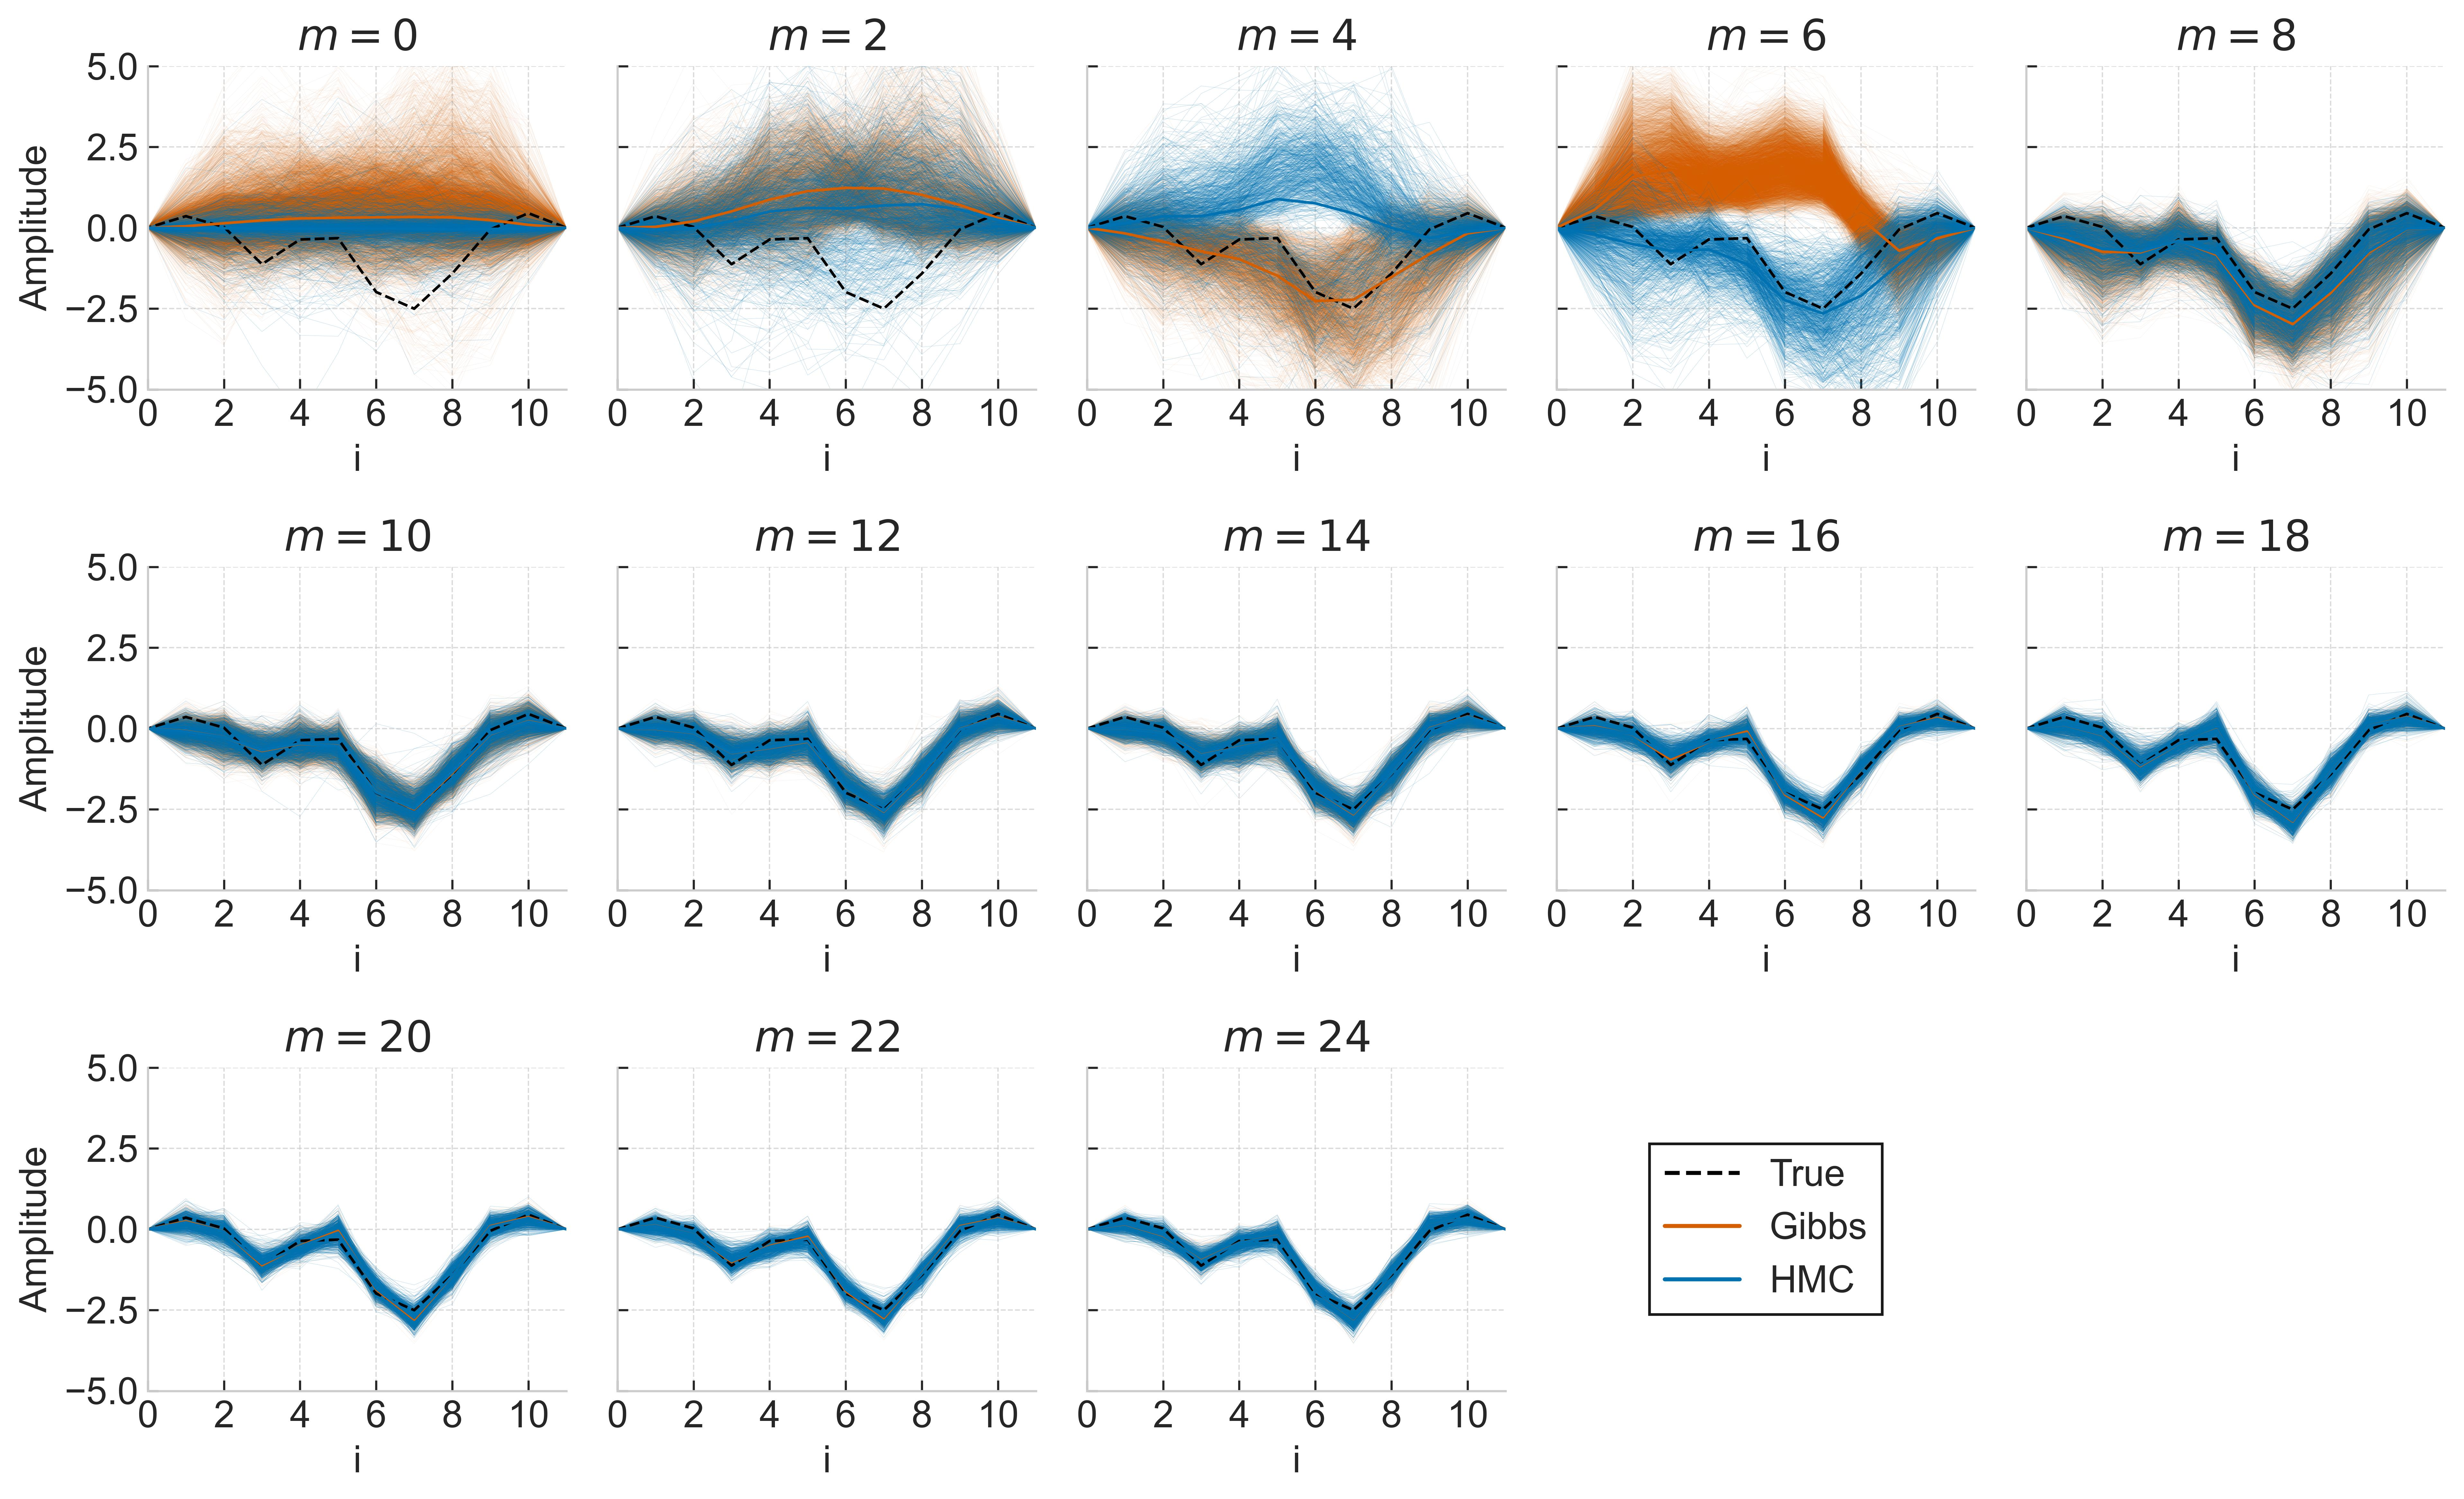
\includegraphics[width=0.95\textwidth, trim=0cm 0cm 0cm 0cm]{images/results/n_pix/posterior_wavelets_k12_nv24_nh1_mv12_m0_seeddata1_seed7635_initRandom_marc_L40_ar05_long_ess_normalized.jpeg}
    \caption{Posterior blur samples, obtained with $\alpha=0$ (Gibbs) and $\alpha=1$ (HMC) in Algorithm~\ref{alg:hybrid}, for the 13 inverse crime experiments considering an increasing number $m$ of exact image observations. Each solid line represents a posterior sample and the dashed black line represent the true simulated blur. Under sign-shift multimodality ($m \leq 8$), Gibbs fails to visit the largest mode, or struggles switching between the modes.}
    \label{fig:posterior_blur_constraints}
\end{figure}

Figure~\ref{fig:ESS_constraints} sheds more light onto the posterior multimodality as a function of $m$. In the figure, we compare the mixing behaviour obtained with $\alpha=0$ and $\alpha=1$, using ESS and mean square jumping distance (MSJD) distributions, the latter given as $\mbox{MSJD}=\sum_{j=1}^{N}(\theta_{i}^{(j)}- \theta_{i}^{j-1})^2/N$ and both computed coordinate-wise for all parameters using $N=45000$ iterations after burn-in.

In Figure~\ref{fig:ESS_constraints_a} we observe that the ESS for $m\leq 8$ 
is larger for HMC. 
When $m=10$ and the number of exact image observations matches the length $k=10$ of the effective blur, significantly destroying the multimodality, there is a sudden increase in the ESS. 
In Figure~\ref{fig:ESS_constraints_c} we observe that HMC consistently matches or outperforms Gibbs in terms of MSJD for all parameters, especially in the hypothesized multimodal regime. 
We interpret that, for our model, 
% , for a small number of image constraints, 
HMC is more adequate for sampling multimodal geometries. 
However, when $m$  is large enough so that the solution space becomes adequately constrained, Gibbs is preferable over HMC due both to a higher raw ESS and ESS per minute, at least for the size of the latter considered.
\begin{figure}[htbp]
    \centering
    \begin{subfigure}[b]{0.45\textwidth}
        \centering
        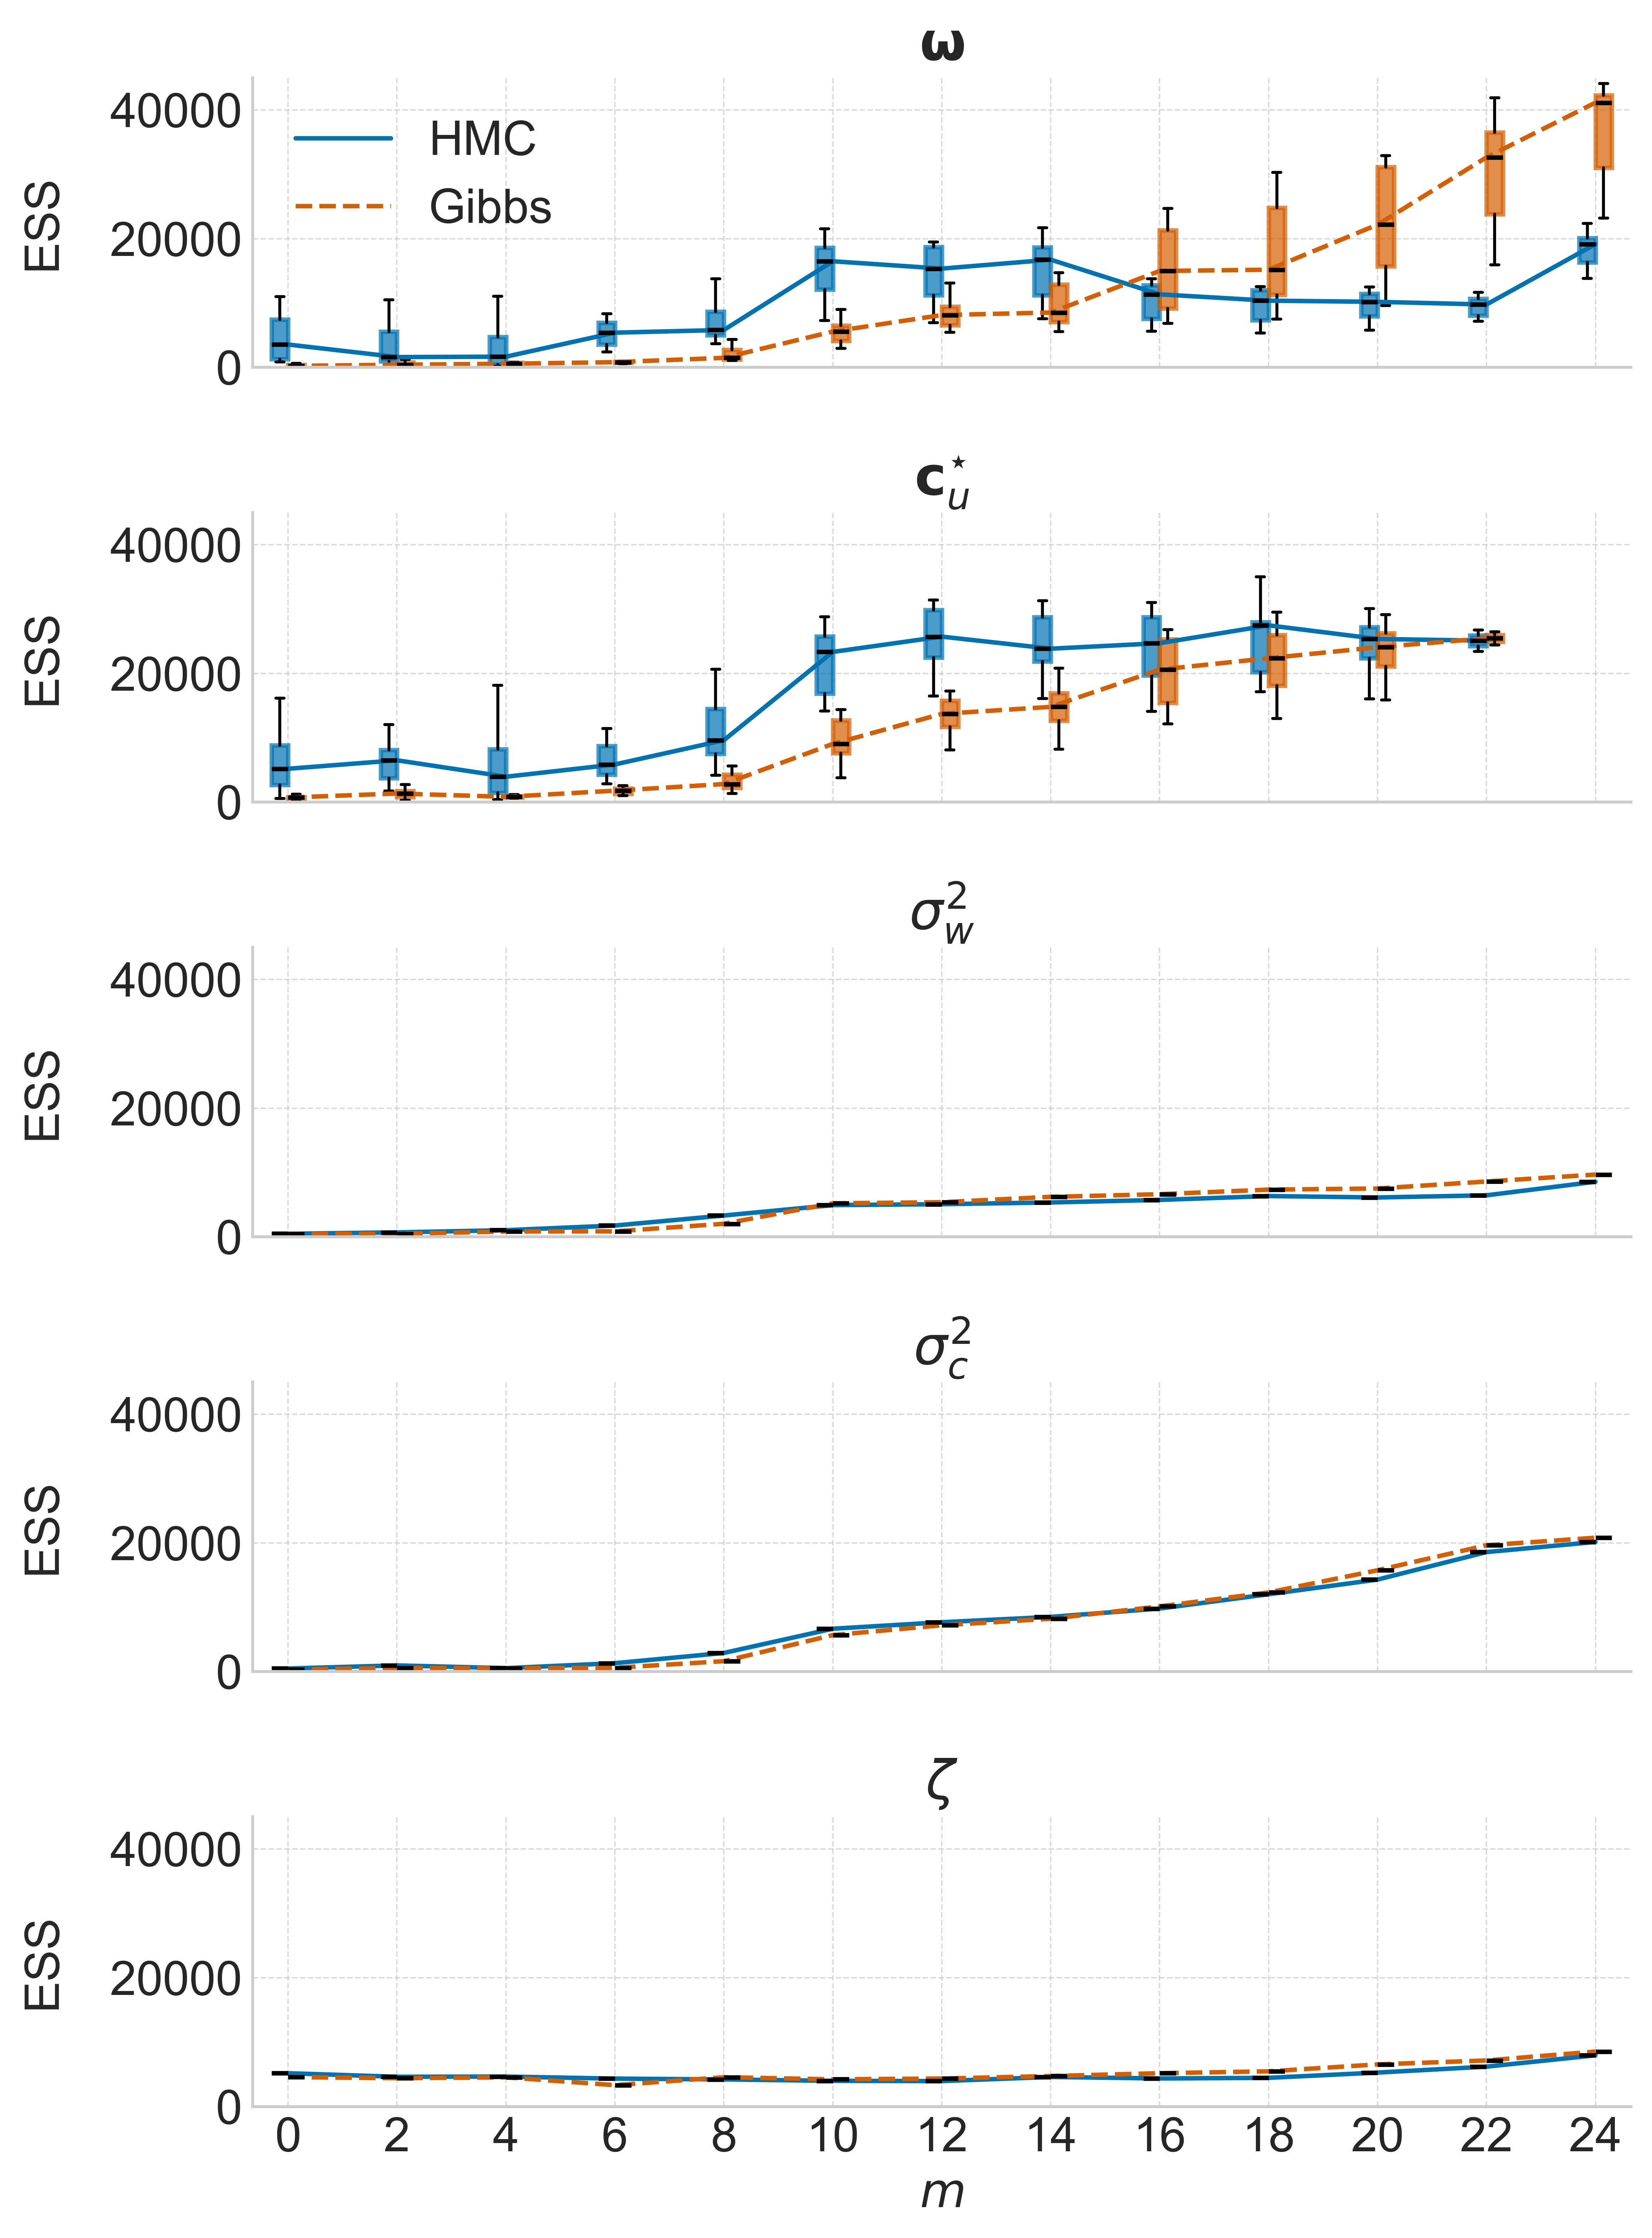
\includegraphics[width=\textwidth]{images/results/n_pix/ess_raw_star_k12_nv24_nh1_mv12_m0_seeddata1_seed7635_initRandom_marc_L40_ar05_long.jpeg}
        \caption{ESS.}
        \label{fig:ESS_constraints_a}
    \end{subfigure}
    \hfill
    \begin{subfigure}[b]{0.45\textwidth}
        \centering
        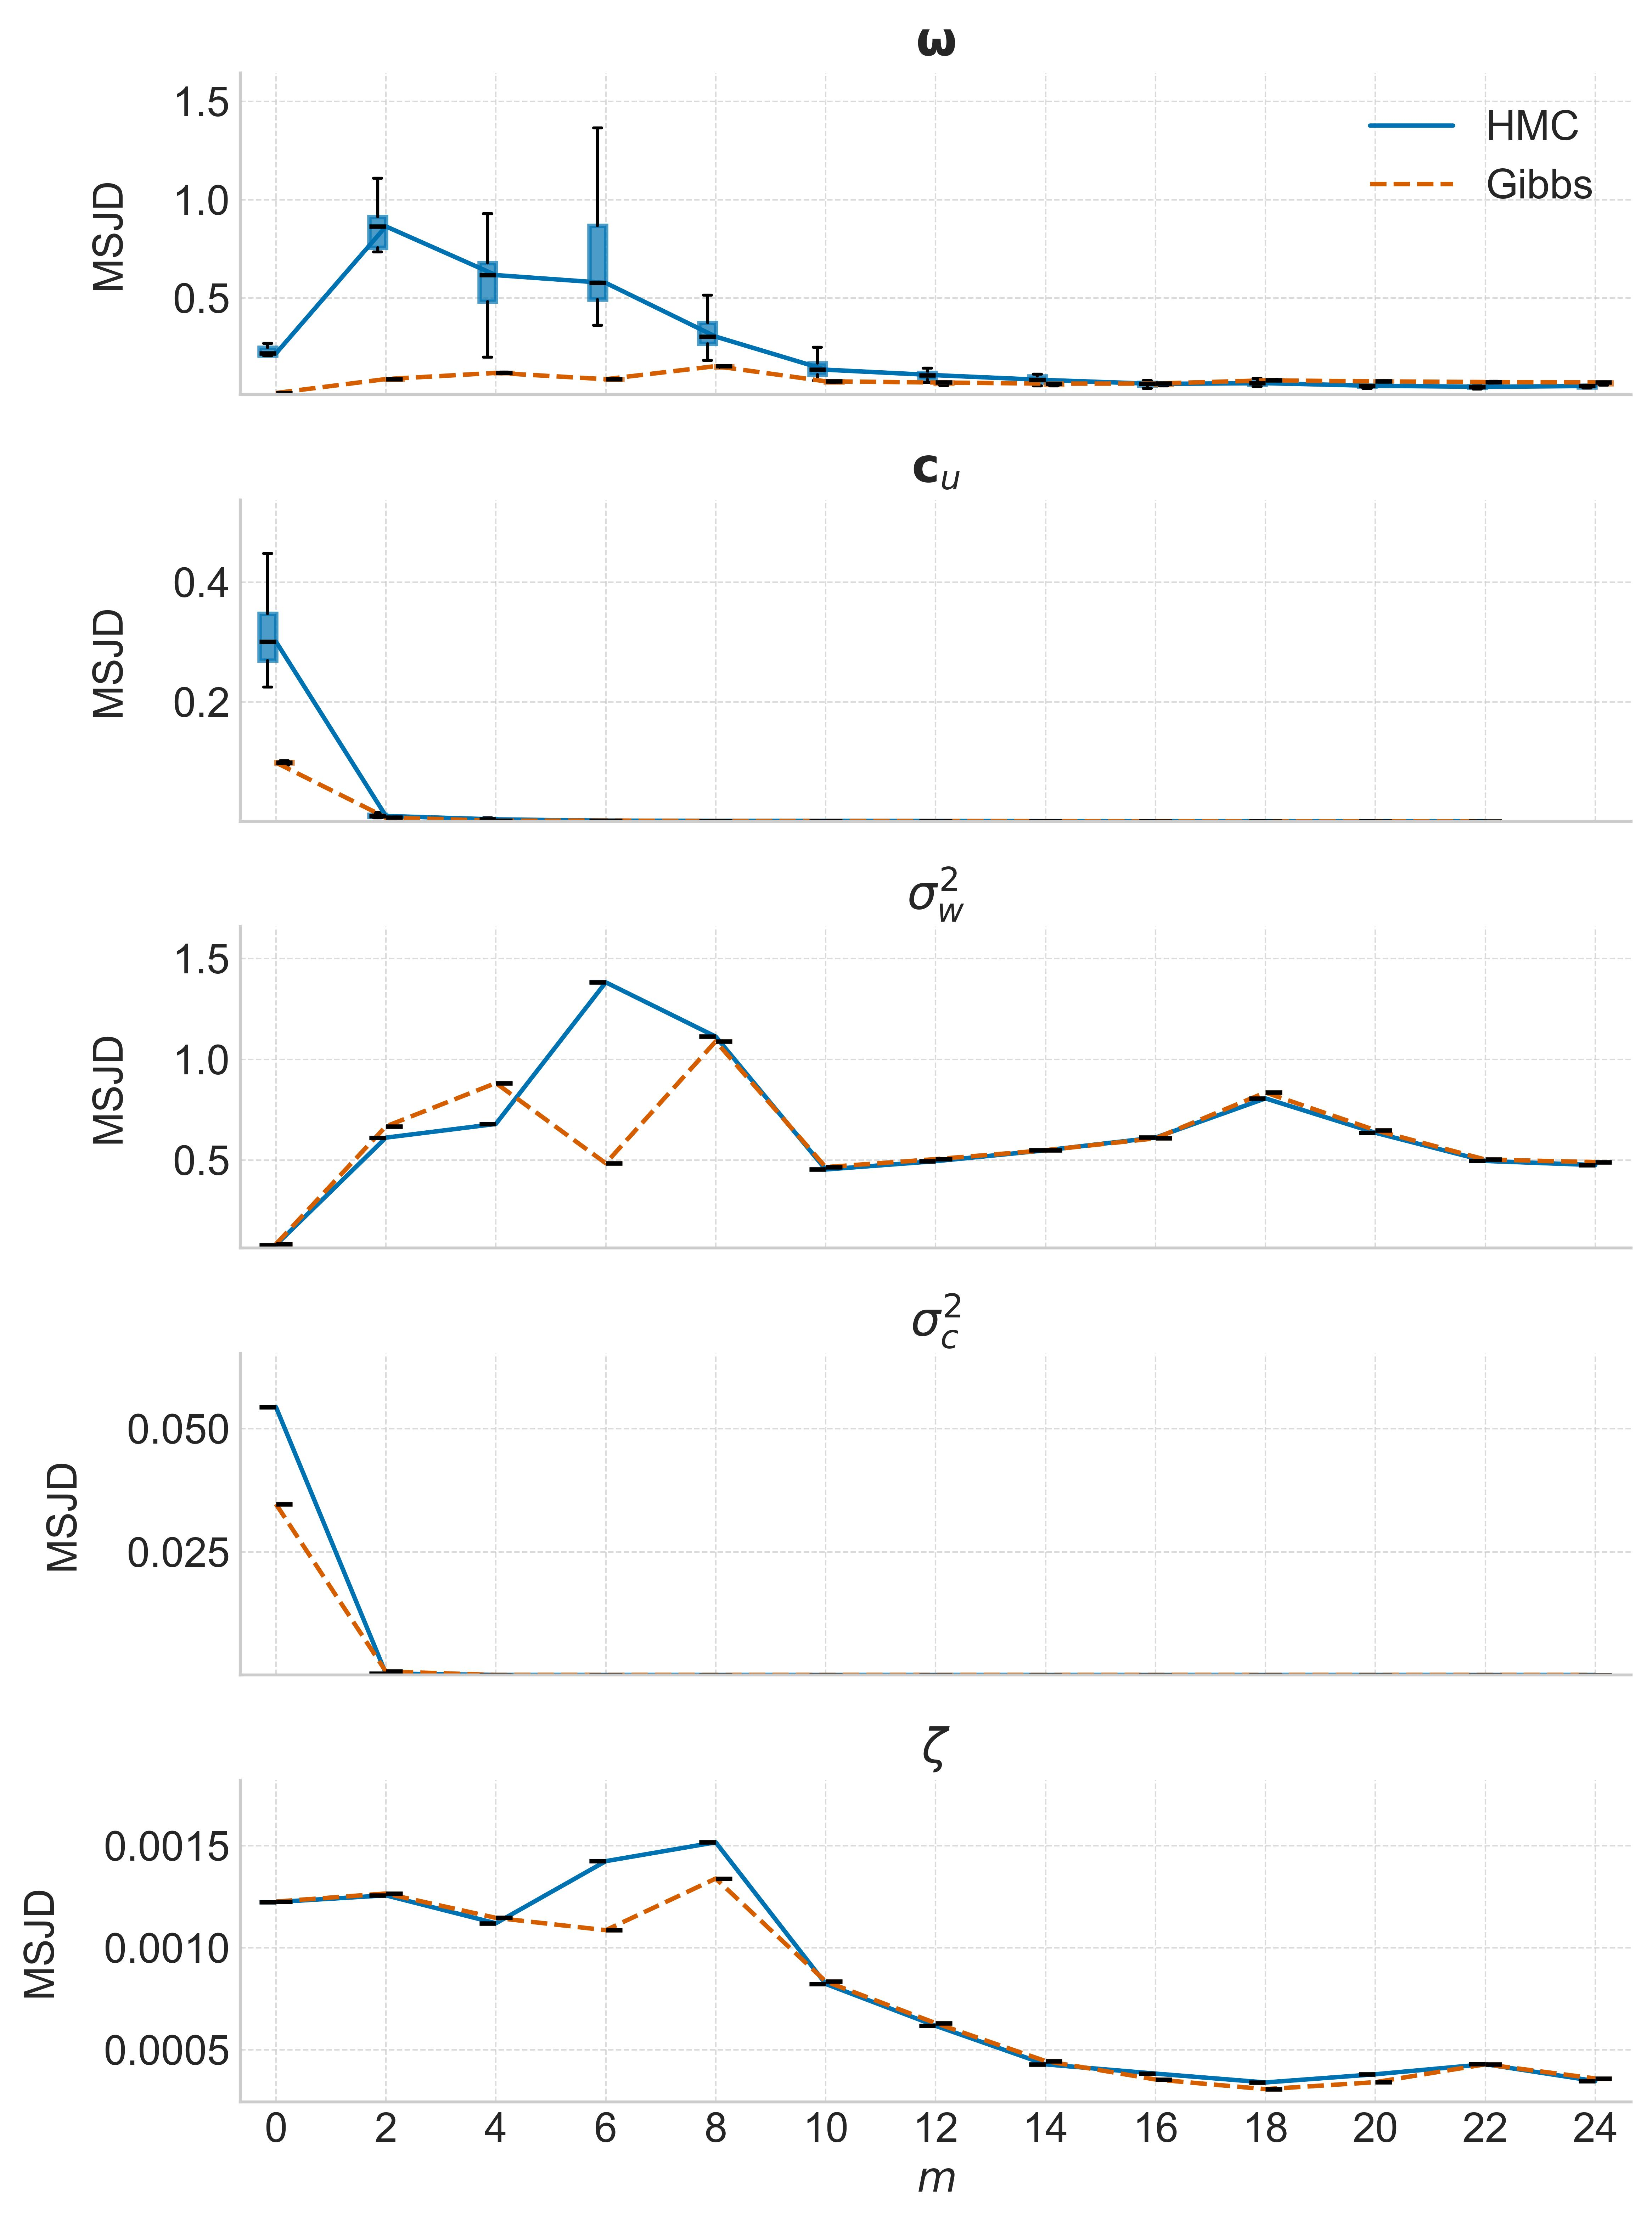
\includegraphics[width=\textwidth]{images/results/n_pix/msjd_k12_nv24_nh1_mv12_m0_seeddata1_seed7635_initRandom_marc_L40_ar05_long.jpeg}
        \caption{MSJD.}
        \label{fig:ESS_constraints_c}
    \end{subfigure}
    \caption{ESS and MSJD distributions for all parameters as a function of the number of exact image observations $m$, for $\alpha=0$ and $\alpha=1$. The HMC blur update induces better ability to jump between the modes in the multimodal regime, while using Gibbs might achieve equal or improved exploration when the solution space is adequately constrained.}
    \label{fig:ESS_constraints}
\end{figure}


\subsection{A large-scale seismic semi-blind deconvolution example}
\label{sec:egypt}

We now consider a real SBD problem in gas reservoir characterization with approximately 80k unknown parameters and 330 exact image observations incorporated as hard constraints. 
Figure~\ref{fig:egypt_data_wavelet_posterior}  shows the $330\times50$ amplitude-versus-offset seismic reflectivity image and the 330 exact well-reflectivity observations located at column 25.  
The gas reservoir is visible in the seismic image near $(x,t)\approx(25,150)$, matching the large-amplitude reflectivity values in the well-log around $t=150$ms.
Details on the seismic acquisition, physical interpretation, and exact image observations are given in Section~\ref{app:seismic_details} in the SM.

\begin{figure}
\centering
\begin{subfigure}[b]{0.5\textwidth}
    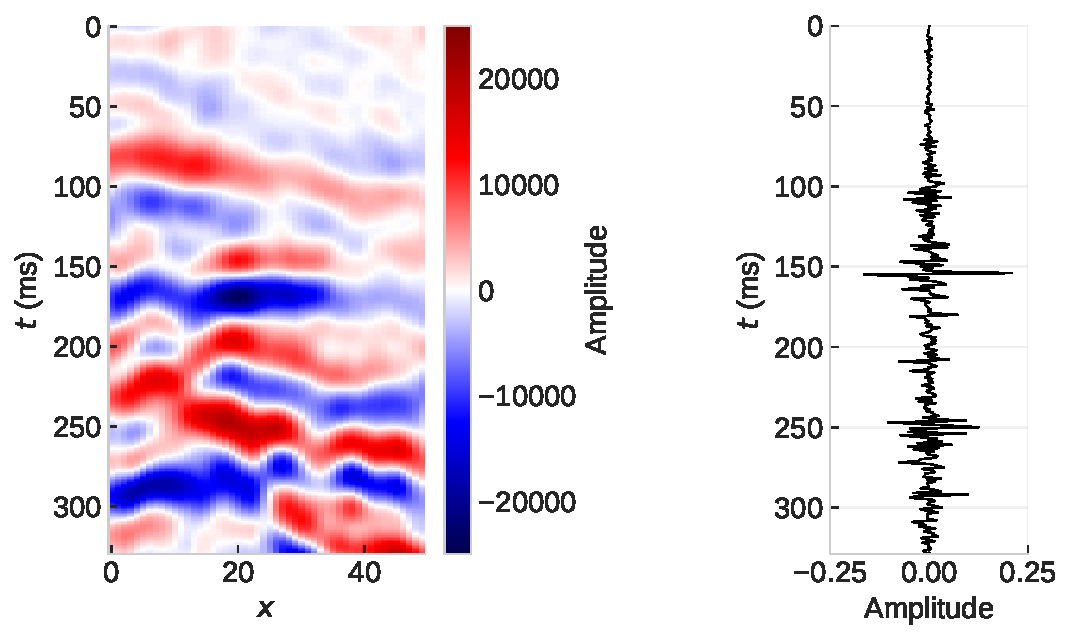
\includegraphics[trim={0 0 0 0}, clip]{images/results/real/20251231_data_well.pdf}
\end{subfigure}
\hfill
\begin{subfigure}[b]{0.4\textwidth}
    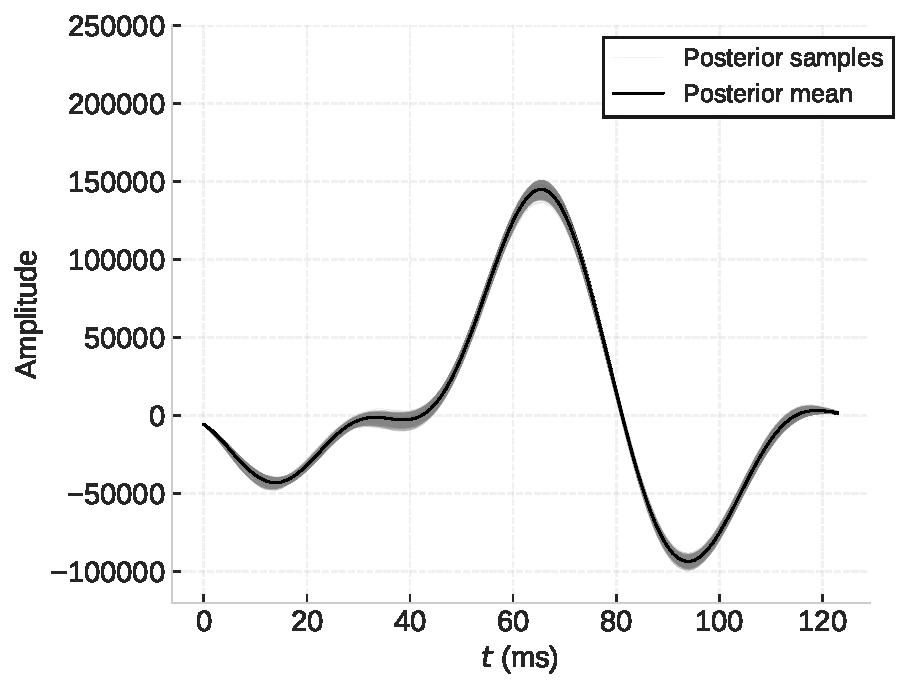
\includegraphics{images/results/real/20251231_wavelet_posterior_480x100_comparisonL_10_20.pdf}
\end{subfigure}
\caption{Left: amplitude-versus-ofset seismic reflectivity image. Middle: analytical well reflectivity. Right: samples from the seismic wavelet posterior distribution.}
\label{fig:egypt_data_wavelet_posterior}
\end{figure}

For the estimation we used the model in Section~\ref{sec:model} with padding $(m_v,m_h)=(150,50)$, determined empirically for the SBD model via a rule of thumb based on the RMSE stabilization (see Section~\ref{sec:margins} in the SM), which yields a $480\times100$ extended lattice. We chose $k=126$ and used the same fixed hyperparameter values as \citet{Senn2025}. We run two single chains, with $3$ million samples for $\alpha=0$ and $100$k samples for $\alpha=1$, both initialized from the same prior realization.
For $\alpha=1$, we set $L=10$ based on preliminary runs and adapted $\varepsilon$ using an ad-hoc tuning procedure. 

Figure~\ref{fig:egypt_traceplots} compares the first iterations of the traceplots for all the parameters and illustrates the burn-in phase, whose end we estimate at iteration 80k for $\alpha=0$ and at iteration 5k for $\alpha=1$. The remaining unplotted iterations showed no evidence of multimodality. At an average computational time per iteration of 0.47s  for $\alpha=0$ and 13s  for $\alpha=1$, the total burn-in computational time was approximately of 10.4 and 18.4 hours, respectively.

\begin{figure}
\centering
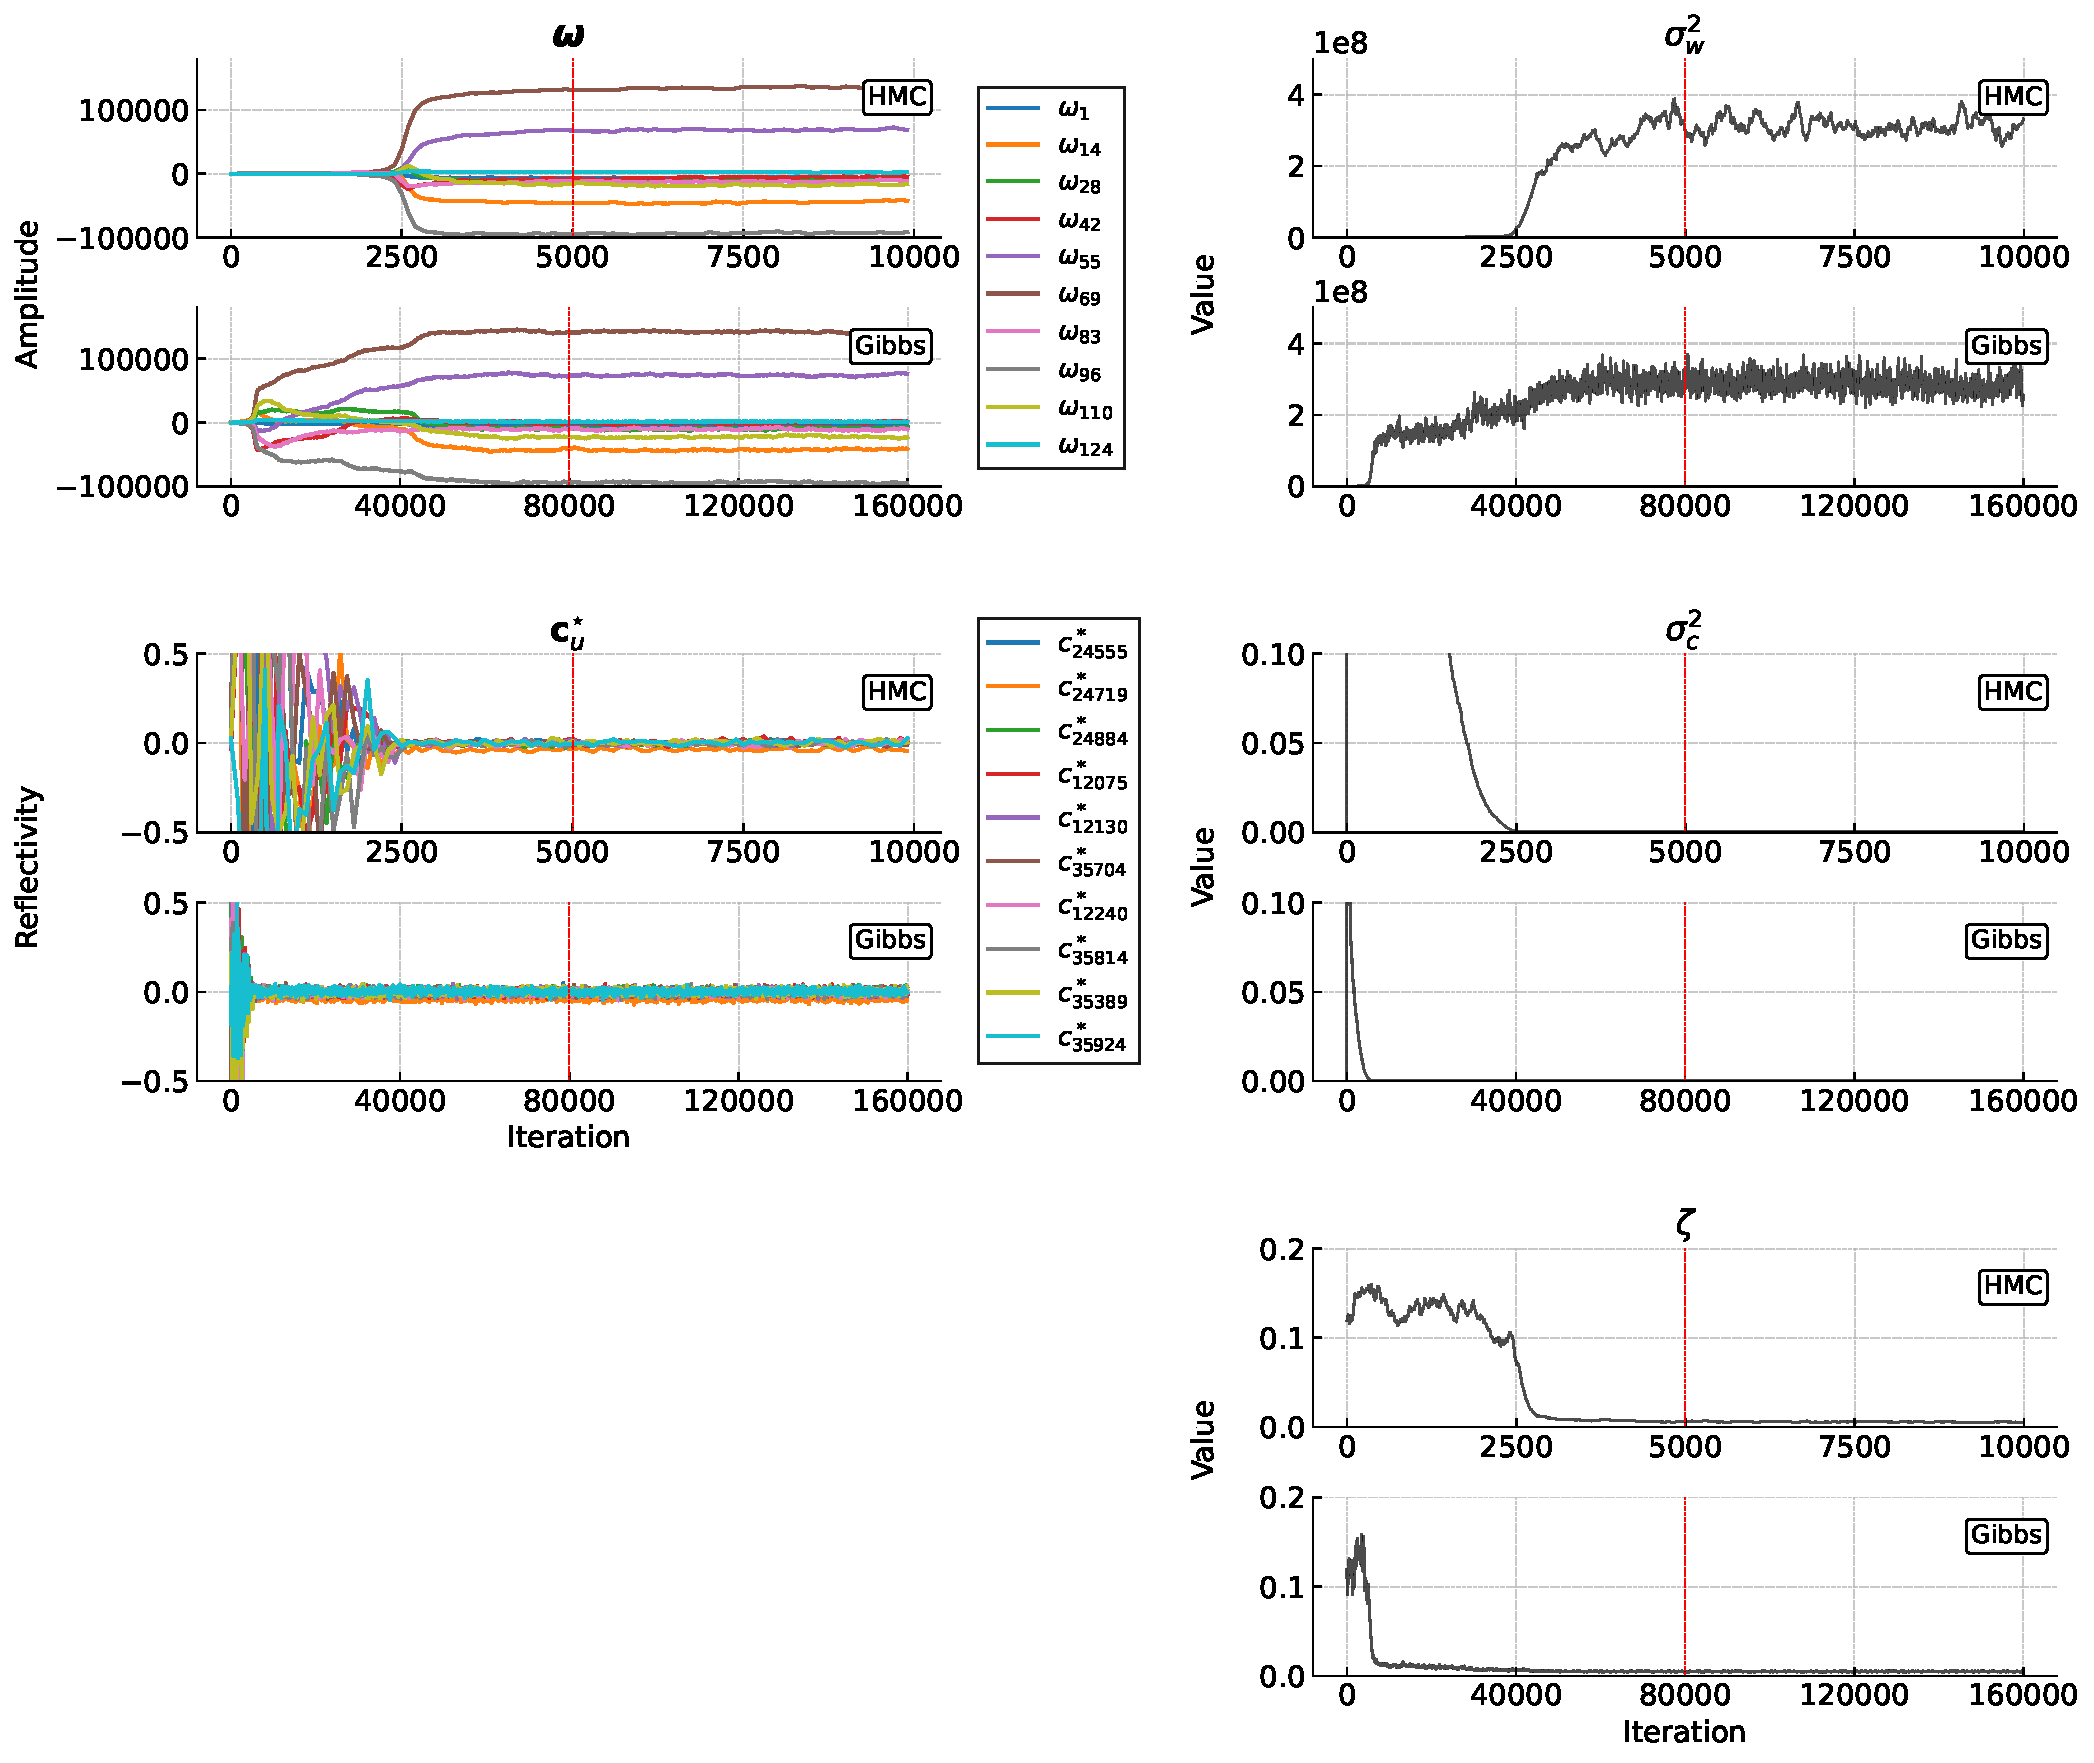
\includegraphics[width=1\textwidth]{images/results/real/20251230_traceplots_Gibbs_HMC_480x100.pdf}
\caption{Traceplots for for 10 elements of each of the multivariate parameters $\bm{\omega}$ and $\bm{c}^\star_u$ and for the univariate parameters $\sigma_w^2$, $\sigma_c^2$, and $\zeta$ in the real example, obtained with Algorithm~\ref{alg:hybrid} using $\alpha=0$ and $\alpha=1$. The burn-in periods are indicated by the vertical red lines.}
\label{fig:egypt_traceplots}
\end{figure}

Table~\ref{table:ess} compares the mixing behaviour of the algorithms through the ESS and MSJD. Both metrics are computed using $N=55$k post-burn-in samples, with ESS estimated up to lag 1500. Apart from some differences, the metrics are broadly comparable across algorithms. However, after accounting for the computational cost per iteration (approximately 25:1 in favour of Gibbs), the ESS per minute is substantially larger for Gibbs.

\begin{table}[ht]
\centering
\scriptsize
\renewcommand{\arraystretch}{1.1}
\setlength{\tabcolsep}{3pt}
\begin{tabular}{lcccc}
 & \multicolumn{2}{c}{\small Effective Sample Size} & \multicolumn{2}{c}{\small Mean Squared Jumping Distance} \\
 & $\alpha=0$ (Gibbs) & $\alpha=1$ (HMC) & $\alpha=0$ (Gibbs)& $\alpha=1$ (HMC)\\
\midrule
$\bm{\omega}$        & 32 (24, 34) & \textbf{133 (119, 146)} & 2.55e+04 (2.54e+04, 2.56e+04) & \textbf{9.77e+04 (9.71e+04, 9.88e+04)} \\
$\bm{c}_u^{\star}$   & 45165 (43032, 47431) & \textbf{46283 (43700, 48224)} & \textbf{0.00028 (0.000279, 0.000281)} & 0.000258 (0.000257, 0.000259) \\
$\sigma^2_c$    & \textbf{44529} & 7116 & \textbf{2.09e-12} & 1.77e-12 \\
$\sigma^2_w$    & \textbf{234} & 145 & 7.09e+12 & \textbf{7.15e+12} \\
$\zeta$         & \textbf{250} & 108 & 2.04e-09& \textbf{2.43e-09} \\
\end{tabular}
\caption{ESS and MSJD for the model parameters obtained with $\alpha=0$ and $\alpha=1$ for the real example. Values represent the median with 2.5th and 97.5th percentiles in parentheses for the multivariate parameters. The values are mostly comparable across algorithms.}
\label{table:ess}
\end{table}

Figure~\ref{fig:egypt_data_wavelet_posterior} (right) illustrates the posterior marginal blur distribution using 4000 randomly selected post-burnin samples from each algorithm. The posterior samples are smooth and almost zero-phase, with narrow $95\%$ posterior intervals indicating low uncertainty. 

Figure~\ref{fig:egypt_posterior_reflectivity} illustrates the posterior marginal image distribution. The posterior mean resembles a denoised version of the observed image, while individual realizations exhibit greater variability. The posterior standard deviation is smallest near the locations where exact image observations are available and increases with distance from them, reflecting the propagation of information through the prior model.

The very low uncertainty in the marginal posterior distribution of the estimated seismic wavelet is surprising from a geophysical perspective.
Typically, wavelets estimated at different well locations within the same dataset would have differences with magnitude larger than the variance of the posterior estimate shown in Figure~\ref{fig:egypt_data_wavelet_posterior} (right) \citep{EdgarVanDerBaan2011}.
\citet{Senn2025} investigated the effect of some model errors on the Gibbs version of the algorithm, and showed that a limited set of such errors affected the magnitude of the posterior variance estimated for the wavelet, although the results were not conclusive. 
The present results suggest that the unexpectedly low posterior uncertainty may be driven by model misspecification. As described in Section~\ref{app:seismic_details} in the SM, we expect there to be significant epistemic errors in the data. For instance, data processing might have failed to make the image a perfect match to the ideal data that could be modeled using the convolutional model, i.e., to make the wavelet stationary. We also expect there to be well alignment errors. 
Model errors are also possibly in the prior distributions. For example, it is reasonable to expect a non-Gaussian reflectivity.

\begin{figure}[bt]
\centering
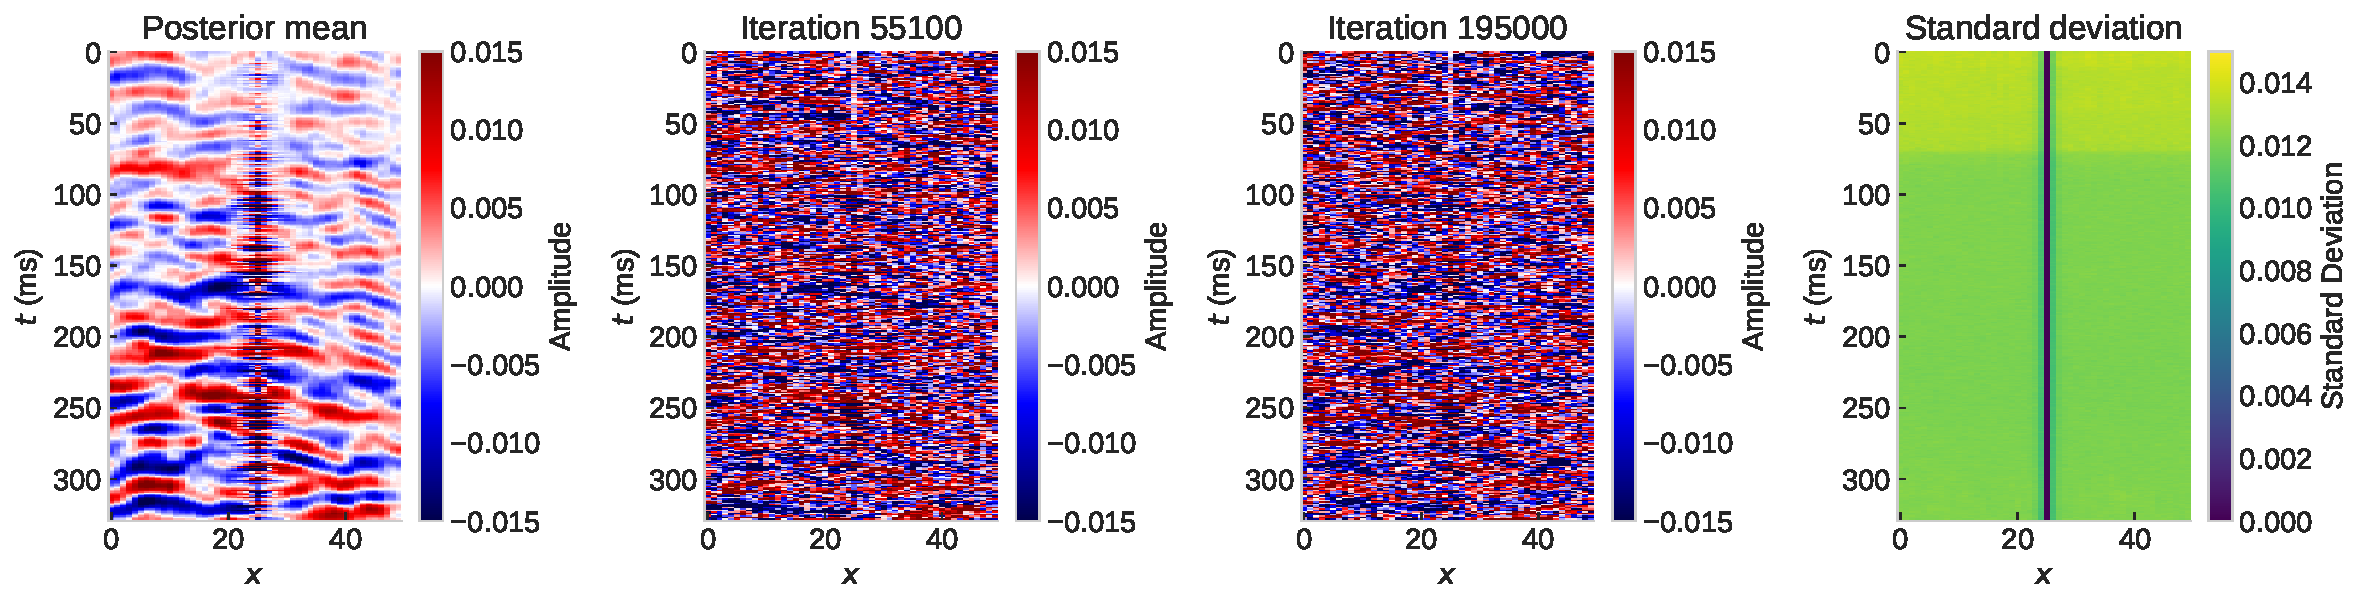
\includegraphics[width=\textwidth]{images/results/real/20251231_reflectivity_posterior_gibbs_HMC_330x50_L10.pdf}
\caption{Mean, two realizations, and standard deviation of samples from the posterior reflectivity image distribution for the real example.}
\label{fig:egypt_posterior_reflectivity}
\end{figure}


\section{Concluding remarks}\label{sec:conclusion}

The simulation study showed that the marginal HMC blur update improves exploration upon the Gibbs conditional update when the SBD posterior is multimodal due to insufficient exact image observations. As the number of exact observations increases and the solution space becomes more constrained, the Gibbs blur update becomes preferable, giving comparable exploration at much lower computational cost.

The real-data example, involving a $330 \times 50$ seismic amplitude-versus-offset dataset with $m=330$ exact well-log reflectivities, overall confirmed the conclusions from the simulation study. The Gibbs and HMC blur updates gave comparable ESS and MSJD values, suggesting that the posterior geometry in this example can be explored efficiently by the pure Gibbs sampler, at a cost of 0.47s per iteration. This also shows that the proposed methodology remains feasible for a realistic large-scale SBD problem with approximately 80k unknown parameters.

The real-data example also revisits the low posterior uncertainty in the estimated seismic wavelet observed by \citet{Senn2025}. Since the alternative HMC blur update leads to similar posterior uncertainty, the low variance does not seem to be related to an inefficient or slow MCMC exploration but rather be a model feature. This suggests an interesting direction for future work, namely to investigate more systematically how assumptions in the forward, prior and noise models affect the posterior uncertainty in the estimated wavelet.

{\spacingset{1}
\bibliography{bibliography.bib}
}

\section{Disclosure statement}\label{disclosure-statement}
The authors have no conflicts of interest to declare.

\section{Data availability statement}
Simulated data and code are provided at \url{https://github.com/to-be-disclosed-after-peer-review}. Real data is not available publicly due to commercial restrictions.

\section*{Acknowledgements}
To be updated after peer-review.

\phantomsection\label{supplementary-material}
\bigskip

\end{document}
